\documentclass[12pt, a4paper]{article}
\usepackage[utf8]{inputenc}
\usepackage{array}
\usepackage[spanish]{babel} 
\usepackage[margin=1.8cm]{geometry}
\usepackage{graphicx}
\usepackage{needspace}
\usepackage[
    colorlinks=true,
    linkcolor=blue,
    filecolor=magenta,
    urlcolor=blue,
    citecolor=blue
]{hyperref}

\newcolumntype{C}[1]{>{\centering\arraybackslash}m{#1}}
\newcolumntype{L}[1]{>{\raggedright\arraybackslash}m{#1}}

\begin{document}


%=================== PORTADA ====================
\section{Portada}
\begin{center}
    \vspace*{2cm}
    {\bfseries\Large Sistema de Gestión de Inventario\par}

    \vspace{0.4cm}
    {\large Documentación del Producto Mínimo Viable (MVP) --- Versión 1.0\par}

    \vspace{2cm}
    Josue Ventura Gutierrez\par
    Andres Josue Luna Escobar\par
    Piter Neytan Eduardo Crispin Salluco\par
    Jhon Beymar Muriel Huaynoca\par

    \vspace{2cm}
    Facultad de Ingeniería en Sistemas\par
    Universidad Adventista de Bolivia\par

    \vspace{1cm}
    
\includegraphics[width=4cm]{doc/imagenes/logo_uab.jpeg}

    \vspace{1cm}
    Ingeniera: Monica Cruz Yauripara\par

    \vspace{1cm}
    \today\par
\end{center}
\newpage

%=================== INDICE ====================
\section{Índice}
\renewcommand{\contentsname}{}
\tableofcontents
\newpage

%=================== ALCANCE DEL MVP ====================
\section{Alcance del MVP}

\subsection{Objetivo}
El objetivo de este Producto Mínimo Viable (MVP) es ofrecer un sistema web que permita a un
pequeño negocio controlar su inventario: registrar productos y categorías, registrar las entradas
de stock (compras a proveedores), visualizar alertas cuando el stock baja del mínimo, consultar y
filtrar el inventario, y auditar el historial de movimientos. El sistema distingue dos roles
(Administrador y Vendedor) y autentica a los usuarios mediante correo y contraseña.

\subsection{Alcance incluido (versión 1.0)}
\begin{itemize}
    \item Autenticación de usuarios con correo y contraseña, cierre de sesión y refresco de token.
    \item Registro de usuarios Administrador y Vendedor, con jerarquía Vendedor $\rightarrow$ Administrador.
    \item Gestión de categorías de productos (crear, listar, editar y eliminar).
    \item Registro y actualización de productos (nombre, categoría, precio, stock mínimo y cantidad inicial).
    \item Registro de entradas de stock (compras a proveedores).
    \item Cálculo automático del stock a partir de los movimientos (entradas menos salidas).
    \item Alerta visual de stock bajo en el panel principal.
    \item Consulta y filtrado del inventario, y consulta del historial de movimientos.
    \item Resumen del día (total de entradas y salidas).
\end{itemize}

\subsection{Fuera del alcance (versión 1.0)}
Quedan fuera de esta primera versión, y se detallan en la sección \emph{Backlog / Fuera del alcance
del MVP}: el registro de salidas/ventas con canal de venta, las estadísticas por período y el
ranking de más vendidos, la gestión avanzada de usuarios (editar, activar/desactivar, cambiar rol),
el CRUD de proveedores por interfaz, la configuración del sistema, las notificaciones por correo o
mensajería y el bloqueo por intentos fallidos.

\subsection{Arquitectura y tecnologías}
El sistema se organiza en capas:
\begin{itemize}
    \item \textbf{Presentación:} plantillas HTML y JavaScript (módulos ES) servidos por Django.
    \item \textbf{Dominio:} \texttt{core/domain} (entidades, objetos de valor y reglas de negocio).
    \item \textbf{Aplicación:} \texttt{core/application} (casos de uso).
    \item \textbf{Infraestructura:} \texttt{infrastructure/} y las aplicaciones Django en \texttt{apps/}
          (adaptadores, repositorios y modelos ORM).
\end{itemize}
Tecnologías: Django, Django REST Framework, SimpleJWT (tokens JWT almacenados en cookies
\texttt{httpOnly}), base de datos SQLite, y frontend HTML/CSS/JavaScript sin frameworks.

\subsection{Criterio de éxito}
El MVP se considera exitoso si un Administrador puede: iniciar sesión, crear categorías, registrar
productos y entradas de stock, ver las alertas de stock bajo, consultar y filtrar el inventario, y
revisar el historial de movimientos; y si un Vendedor puede iniciar sesión y consultar el inventario
con las restricciones de acceso por rol.

\newpage

%=================== REQUERIMIENTOS FUNCIONALES =====
\section{Requerimientos funcionales}

\subsection{RF-01: Registrar producto}
\begin{center}
\renewcommand{\arraystretch}{1.4}
\begin{tabular}{|L{4cm}|L{12cm}|}
\hline
\textbf{ID} & RF-01 \\
\hline
\textbf{Nombre} & Registrar producto \\
\hline
\textbf{Descripción} & El sistema debe permitir registrar un producto con nombre, categoría, precio unitario, stock mínimo y cantidad inicial, generando automáticamente el movimiento de stock inicial. \\
\hline
\textbf{Actor} & Administrador \\
\hline
\textbf{Entradas} & Nombre, Categoría, Precio unitario, Stock mínimo, Cantidad inicial \\
\hline
\textbf{Salidas} & Producto registrado en la base de datos, Movimiento de entrada con motivo ``Stock inicial'' generado \\
\hline
\textbf{Precondiciones} & El administrador debe estar autenticado, Debe existir al menos una categoría registrada (RF-12) \\
\hline
\textbf{Postcondiciones} & El producto queda disponible para registrar entradas y salidas, El producto aparece en la lista de productos (RF-06) \\
\hline
\textbf{Prioridad (MoSCoW)} & Must \\
\hline
\textbf{CU relacionado} & CU-002 \\
\hline
\end{tabular}
\end{center}

\subsection{RF-02: Registrar entrada de stock}
\begin{center}
\renewcommand{\arraystretch}{1.4}
\begin{tabular}{|L{4cm}|L{12cm}|}
\hline
\textbf{ID} & RF-02 \\
\hline
\textbf{Nombre} & Registrar entrada de stock \\
\hline
\textbf{Descripción} & El sistema debe permitir registrar una entrada de stock (compra a proveedor) indicando producto, cantidad y proveedor. El proveedor es una entidad registrada (no un texto libre). \\
\hline
\textbf{Actor} & Administrador \\
\hline
\textbf{Entradas} & Producto, Cantidad, Proveedor \\
\hline
\textbf{Salidas} & Movimiento de entrada (motivo ``Compra a proveedor'') registrado con fecha y hora, Stock del producto recalculado \\
\hline
\textbf{Precondiciones} & El administrador debe estar autenticado, El producto debe existir (RF-01), El proveedor debe existir y estar activo \\
\hline
\textbf{Postcondiciones} & El stock calculado del producto queda actualizado, El movimiento queda registrado en el historial (RF-08) \\
\hline
\textbf{Prioridad (MoSCoW)} & Must \\
\hline
\textbf{CU relacionado} & CU-003 \\
\hline
\end{tabular}
\end{center}

\subsection{RF-03: Actualizar producto}
\begin{center}
\renewcommand{\arraystretch}{1.4}
\begin{tabular}{|L{4cm}|L{12cm}|}
\hline
\textbf{ID} & RF-03 \\
\hline
\textbf{Nombre} & Actualizar producto \\
\hline
\textbf{Descripción} & El sistema debe permitir modificar los datos de un producto existente (nombre, categoría, precio unitario y stock mínimo). \\
\hline
\textbf{Actor} & Administrador \\
\hline
\textbf{Entradas} & Identificador del producto, Datos actualizados \\
\hline
\textbf{Salidas} & Producto actualizado en la base de datos \\
\hline
\textbf{Precondiciones} & El administrador debe estar autenticado, El producto debe existir \\
\hline
\textbf{Postcondiciones} & Los cambios quedan reflejados en la lista de productos (RF-06) \\
\hline
\textbf{Prioridad (MoSCoW)} & Should \\
\hline
\textbf{CU relacionado} & CU-016 \\
\hline
\end{tabular}
\end{center}

\subsection{RF-04: Cálculo automático del stock}
\begin{center}
\renewcommand{\arraystretch}{1.4}
\begin{tabular}{|L{4cm}|L{12cm}|}
\hline
\textbf{ID} & RF-04 \\
\hline
\textbf{Nombre} & Cálculo automático del stock \\
\hline
\textbf{Descripción} & El sistema debe calcular la cantidad disponible de un producto a partir de sus movimientos (suma de entradas menos suma de salidas), sin necesidad de actualizaciones manuales. \\
\hline
\textbf{Actor} & Sistema \\
\hline
\textbf{Entradas} & Movimientos de entrada y salida del producto \\
\hline
\textbf{Salidas} & Cantidad disponible calculada \\
\hline
\textbf{Precondiciones} & Debe existir al menos un movimiento asociado al producto \\
\hline
\textbf{Postcondiciones} & El stock refleja el valor correcto tras cada movimiento, Se recalcula el estado de alerta \\
\hline
\textbf{Prioridad (MoSCoW)} & Must \\
\hline
\textbf{CU relacionado} & CU-002, CU-003, CU-005 \\
\hline
\end{tabular}
\end{center}

\subsection{RF-05: Alerta visual de stock bajo}
\begin{center}
\renewcommand{\arraystretch}{1.4}
\begin{tabular}{|L{4cm}|L{12cm}|}
\hline
\textbf{ID} & RF-05 \\
\hline
\textbf{Nombre} & Alerta visual de stock bajo \\
\hline
\textbf{Descripción} & El sistema debe mostrar una alerta visual en el panel principal cuando el stock de un producto sea igual o inferior al mínimo configurado. La notificación por correo o mensajería queda fuera del alcance de esta versión. \\
\hline
\textbf{Actor} & Sistema \\
\hline
\textbf{Entradas} & Stock calculado del producto, Stock mínimo configurado \\
\hline
\textbf{Salidas} & Lista de productos en alerta mostrada en el panel principal \\
\hline
\textbf{Precondiciones} & El producto debe estar activo y tener configurado un stock mínimo \\
\hline
\textbf{Postcondiciones} & El producto aparece marcado en el panel mientras su stock sea menor o igual al mínimo \\
\hline
\textbf{Prioridad (MoSCoW)} & Must \\
\hline
\textbf{CU relacionado} & CU-005 \\
\hline
\end{tabular}
\end{center}

\subsection{RF-06: Consultar lista de productos}
\begin{center}
\renewcommand{\arraystretch}{1.4}
\begin{tabular}{|L{4cm}|L{12cm}|}
\hline
\textbf{ID} & RF-06 \\
\hline
\textbf{Nombre} & Consultar lista de productos \\
\hline
\textbf{Descripción} & El sistema debe permitir consultar la lista de productos con su stock calculado. \\
\hline
\textbf{Actor} & Administrador / Vendedor \\
\hline
\textbf{Entradas} & Solicitud de consulta de productos \\
\hline
\textbf{Salidas} & Lista de productos con nombre, categoría, precio, stock y stock mínimo \\
\hline
\textbf{Precondiciones} & El usuario debe estar autenticado \\
\hline
\textbf{Postcondiciones} & Se muestra la información sin modificar el sistema \\
\hline
\textbf{Prioridad (MoSCoW)} & Must \\
\hline
\textbf{CU relacionado} & CU-006 \\
\hline
\end{tabular}
\end{center}

\subsection{RF-07: Filtrar productos}
\begin{center}
\renewcommand{\arraystretch}{1.4}
\begin{tabular}{|L{4cm}|L{12cm}|}
\hline
\textbf{ID} & RF-07 \\
\hline
\textbf{Nombre} & Filtrar productos \\
\hline
\textbf{Descripción} & El sistema debe permitir filtrar productos por categoría, nombre y estado de stock, donde: Disponible = stock $>$ stock mínimo; Bajo = 0 $<$ stock $\leq$ stock mínimo; Agotado = stock = 0. \\
\hline
\textbf{Actor} & Administrador / Vendedor \\
\hline
\textbf{Entradas} & Categoría, Nombre, Estado de stock \\
\hline
\textbf{Salidas} & Lista filtrada de productos \\
\hline
\textbf{Precondiciones} & El usuario debe estar autenticado \\
\hline
\textbf{Postcondiciones} & Se muestra la lista filtrada sin modificar el sistema \\
\hline
\textbf{Prioridad (MoSCoW)} & Should \\
\hline
\textbf{CU relacionado} & CU-007 \\
\hline
\end{tabular}
\end{center}

\subsection{RF-08: Consultar historial de movimientos}
\begin{center}
\renewcommand{\arraystretch}{1.4}
\begin{tabular}{|L{4cm}|L{12cm}|}
\hline
\textbf{ID} & RF-08 \\
\hline
\textbf{Nombre} & Consultar historial de movimientos \\
\hline
\textbf{Descripción} & El sistema debe permitir consultar el historial de movimientos de stock (entradas y salidas), ordenado cronológicamente. \\
\hline
\textbf{Actor} & Administrador \\
\hline
\textbf{Entradas} & Producto seleccionado (opcional) \\
\hline
\textbf{Salidas} & Listado cronológico de movimientos: fecha, categoría/producto, cantidad y proveedor \\
\hline
\textbf{Precondiciones} & El usuario debe estar autenticado \\
\hline
\textbf{Postcondiciones} & Se muestra el historial sin modificar el sistema \\
\hline
\textbf{Prioridad (MoSCoW)} & Must \\
\hline
\textbf{CU relacionado} & CU-008 \\
\hline
\end{tabular}
\end{center}

\subsection{RF-09: Consultar resumen del día}
\begin{center}
\renewcommand{\arraystretch}{1.4}
\begin{tabular}{|L{4cm}|L{12cm}|}
\hline
\textbf{ID} & RF-09 \\
\hline
\textbf{Nombre} & Consultar resumen del día \\
\hline
\textbf{Descripción} & El sistema debe mostrar los totales del día: cantidad total de entradas y cantidad total de salidas de stock. \\
\hline
\textbf{Actor} & Administrador / Vendedor \\
\hline
\textbf{Entradas} & Fecha actual \\
\hline
\textbf{Salidas} & Total de entradas y total de salidas del día \\
\hline
\textbf{Precondiciones} & El usuario debe estar autenticado \\
\hline
\textbf{Postcondiciones} & Se muestra el resumen sin modificar el sistema \\
\hline
\textbf{Prioridad (MoSCoW)} & Should \\
\hline
\textbf{CU relacionado} & CU-017 \\
\hline
\end{tabular}
\end{center}

\subsection{RF-10: Registrar usuarios}
\begin{center}
\renewcommand{\arraystretch}{1.4}
\begin{tabular}{|L{4cm}|L{12cm}|}
\hline
\textbf{ID} & RF-10 \\
\hline
\textbf{Nombre} & Registrar usuarios \\
\hline
\textbf{Descripción} & El sistema debe permitir registrar usuarios con dos roles: Administrador y Vendedor. Cada Vendedor queda asociado obligatoriamente a un Administrador. \\
\hline
\textbf{Actor} & Administrador / Registro público \\
\hline
\textbf{Entradas} & Nombre de usuario, Correo, Contraseña, Rol (Administrador / Vendedor), Usuario del administrador (solo para Vendedor) \\
\hline
\textbf{Salidas} & Usuario registrado en la base de datos según su rol \\
\hline
\textbf{Precondiciones} & El correo no debe estar registrado, Para un Vendedor debe existir el Administrador indicado \\
\hline
\textbf{Postcondiciones} & El usuario queda habilitado para iniciar sesión según su rol \\
\hline
\textbf{Prioridad (MoSCoW)} & Must \\
\hline
\textbf{CU relacionado} & CU-013, CU-014 \\
\hline
\end{tabular}
\end{center}

\subsection{RF-11: Control de acceso según rol}
\begin{center}
\renewcommand{\arraystretch}{1.4}
\begin{tabular}{|L{4cm}|L{12cm}|}
\hline
\textbf{ID} & RF-11 \\
\hline
\textbf{Nombre} & Control de acceso según rol \\
\hline
\textbf{Descripción} & El sistema debe dirigir a cada usuario a un panel distinto según su rol: el Administrador accede a todas las secciones de gestión y el Vendedor solo a Inicio e Inventario. Las peticiones a la API requieren autenticación. \\
\hline
\textbf{Actor} & Sistema \\
\hline
\textbf{Entradas} & Rol del usuario autenticado \\
\hline
\textbf{Salidas} & Panel de Administrador o de Vendedor, Acceso denegado a la API sin autenticación \\
\hline
\textbf{Precondiciones} & El usuario debe estar autenticado \\
\hline
\textbf{Postcondiciones} & El usuario accede únicamente a las secciones correspondientes a su rol \\
\hline
\textbf{Prioridad (MoSCoW)} & Must \\
\hline
\textbf{CU relacionado} & CU-001, CU-011 \\
\hline
\end{tabular}
\end{center}

\subsection{RF-12: Gestionar categorías de productos}
\begin{center}
\renewcommand{\arraystretch}{1.4}
\begin{tabular}{|L{4cm}|L{12cm}|}
\hline
\textbf{ID} & RF-12 \\
\hline
\textbf{Nombre} & Gestionar categorías de productos \\
\hline
\textbf{Descripción} & El sistema debe permitir registrar, listar, editar y eliminar categorías de productos. No se podrá eliminar una categoría con productos asociados. \\
\hline
\textbf{Actor} & Administrador \\
\hline
\textbf{Entradas} & Nombre de la categoría \\
\hline
\textbf{Salidas} & Categoría registrada, actualizada o eliminada en el sistema \\
\hline
\textbf{Precondiciones} & El administrador debe estar autenticado \\
\hline
\textbf{Postcondiciones} & La categoría queda disponible para asignar a productos (RF-01) \\
\hline
\textbf{Prioridad (MoSCoW)} & Must \\
\hline
\textbf{CU relacionado} & CU-012 \\
\hline
\end{tabular}
\end{center}

\subsection{RF-13: Autenticación de usuarios}
\begin{center}
\renewcommand{\arraystretch}{1.4}
\begin{tabular}{|L{4cm}|L{12cm}|}
\hline
\textbf{ID} & RF-13 \\
\hline
\textbf{Nombre} & Autenticación de usuarios \\
\hline
\textbf{Descripción} & El sistema debe permitir iniciar sesión con correo y contraseña, cerrar sesión y refrescar el token de acceso. La sesión se gestiona con tokens JWT almacenados en cookies. \\
\hline
\textbf{Actor} & Administrador / Vendedor \\
\hline
\textbf{Entradas} & Correo, Contraseña \\
\hline
\textbf{Salidas} & Tokens de acceso y refresco almacenados en cookies, Sesión cerrada al solicitar logout \\
\hline
\textbf{Precondiciones} & El usuario debe estar registrado (RF-10) \\
\hline
\textbf{Postcondiciones} & El usuario accede al panel correspondiente a su rol \\
\hline
\textbf{Prioridad (MoSCoW)} & Must \\
\hline
\textbf{CU relacionado} & CU-001, CU-015 \\
\hline
\end{tabular}
\end{center}

\newpage

% ==================== REQUERIMIENTOS NO FUNCIONALES ====================
\section{Requerimientos No funcionales}

\subsection{RNF-01: Facilidad de uso para usuarios básicos}
\begin{center}
\renewcommand{\arraystretch}{1.4}
\begin{tabular}{|L{4cm}|L{12cm}|}
\hline
\textbf{ID} & RNF-01 \\
\hline
\textbf{Categoría} & Usabilidad \\
\hline
\textbf{Nombre} & Facilidad de uso para usuarios básicos \\
\hline
\textbf{Descripción} & Un usuario con conocimientos básicos de informática debe poder completar las tareas principales (registrar producto, registrar entrada, consultar stock y ver alertas) sin ayuda externa. \\
\hline
\textbf{Métrica} & Máximo 3 intentos por tarea y menos de 5 minutos por tarea. \\
\hline
\textbf{Criterio de aceptación} & Prueba con al menos 5 usuarios sin experiencia previa, con una tasa de éxito del 80\% o superior. \\
\hline
\textbf{Prioridad (MoSCoW)} & Should \\
\hline
\textbf{CU relacionado} & CU-002, CU-003, CU-005 \\
\hline
\end{tabular}
\end{center}

\subsection{RNF-02: Protección de credenciales y sesiones}
\begin{center}
\renewcommand{\arraystretch}{1.4}
\begin{tabular}{|L{4cm}|L{12cm}|}
\hline
\textbf{ID} & RNF-02 \\
\hline
\textbf{Categoría} & Seguridad \\
\hline
\textbf{Nombre} & Protección de credenciales y sesiones \\
\hline
\textbf{Descripción} & El sistema debe proteger las credenciales de los usuarios y gestionar las sesiones de forma segura. \\
\hline
\textbf{Métrica} & Contraseñas almacenadas con hash PBKDF2 (Django). Tokens JWT en cookies \texttt{httpOnly} con \texttt{SameSite=Lax}; el token de acceso expira en 15 minutos y el de refresco en 7 días. Uso de HTTPS/TLS en producción. \\
\hline
\textbf{Criterio de aceptación} & Revisión de configuración que verifique el hash de contraseñas, las cookies \texttt{httpOnly}, la expiración de tokens y el uso de HTTPS. \\
\hline
\textbf{Prioridad (MoSCoW)} & Must \\
\hline
\textbf{CU relacionado} & CU-001, CU-013, CU-014, CU-015 \\
\hline
\end{tabular}
\end{center}

\subsection{RNF-03: Tiempo de respuesta en consultas y registros}
\begin{center}
\renewcommand{\arraystretch}{1.4}
\begin{tabular}{|L{4cm}|L{12cm}|}
\hline
\textbf{ID} & RNF-03 \\
\hline
\textbf{Categoría} & Rendimiento \\
\hline
\textbf{Nombre} & Tiempo de respuesta en consultas y registros \\
\hline
\textbf{Descripción} & El sistema debe responder en tiempos aceptables bajo carga normal de operación. \\
\hline
\textbf{Métrica} & Con hasta 10.000 productos y 5 usuarios concurrentes: consultas en menos de 2 segundos (percentil 95) y registros en menos de 1 segundo. \\
\hline
\textbf{Criterio de aceptación} & Prueba de carga que simule 10.000 productos y 5 usuarios concurrentes, midiendo el percentil 95 de los tiempos de respuesta. \\
\hline
\textbf{Prioridad (MoSCoW)} & Should \\
\hline
\textbf{CU relacionado} & CU-003, CU-005, CU-006, CU-007, CU-008, CU-017 \\
\hline
\end{tabular}
\end{center}

\subsection{RNF-04: Arquitectura en capas y cobertura de pruebas}
\begin{center}
\renewcommand{\arraystretch}{1.4}
\begin{tabular}{|L{4cm}|L{12cm}|}
\hline
\textbf{ID} & RNF-04 \\
\hline
\textbf{Categoría} & Mantenibilidad \\
\hline
\textbf{Nombre} & Arquitectura en capas y cobertura de pruebas \\
\hline
\textbf{Descripción} & El sistema debe organizarse en capas (dominio, aplicación, infraestructura) y contar con pruebas automatizadas que faciliten su mantenimiento. \\
\hline
\textbf{Métrica} & Separación en capas \texttt{core/domain}, \texttt{core/application}, \texttt{infrastructure} y \texttt{apps/}. Pruebas automatizadas con \texttt{pytest}. Cobertura mínima del 70\% en la capa de lógica de negocio. \\
\hline
\textbf{Criterio de aceptación} & Revisión de la arquitectura que confirme la separación de capas y reporte de cobertura de pruebas $\geq$70\%. \\
\hline
\textbf{Prioridad (MoSCoW)} & Should \\
\hline
\textbf{CU relacionado} & CU-002, CU-003, CU-012 \\
\hline
\end{tabular}
\end{center}

\subsection{RNF-05: Incorporación de nuevos módulos sin reestructuración}
\begin{center}
\renewcommand{\arraystretch}{1.4}
\begin{tabular}{|L{4cm}|L{12cm}|}
\hline
\textbf{ID} & RNF-05 \\
\hline
\textbf{Categoría} & Escalabilidad \\
\hline
\textbf{Nombre} & Incorporación de nuevos módulos sin reestructuración \\
\hline
\textbf{Descripción} & La arquitectura debe permitir incorporar nuevos módulos de integración externa sin afectar el núcleo del sistema. \\
\hline
\textbf{Métrica} & Incorporar un nuevo módulo sin modificar más del 20\% del código existente y sin alterar el modelo de datos central. \\
\hline
\textbf{Criterio de aceptación} & Prueba de incorporación de un módulo simulado, midiendo el porcentaje de código modificado. \\
\hline
\textbf{Prioridad (MoSCoW)} & Could \\
\hline
\textbf{CU relacionado} & --- \\
\hline
\end{tabular}
\end{center}

\subsection{RNF-06: Compatibilidad con navegadores y dispositivos}
\begin{center}
\renewcommand{\arraystretch}{1.4}
\begin{tabular}{|L{4cm}|L{12cm}|}
\hline
\textbf{ID} & RNF-06 \\
\hline
\textbf{Categoría} & Compatibilidad \\
\hline
\textbf{Nombre} & Compatibilidad con navegadores y dispositivos \\
\hline
\textbf{Descripción} & El sistema debe funcionar correctamente en los principales navegadores y dispositivos. \\
\hline
\textbf{Métrica} & Últimas dos versiones estables de Chrome, Firefox, Edge y Safari. Resolución de escritorio ($\geq$1280 px) y móvil ($\geq$360 px). Diseño responsive. \\
\hline
\textbf{Criterio de aceptación} & Pruebas de compatibilidad en los 4 navegadores y en resoluciones de escritorio y móvil. \\
\hline
\textbf{Prioridad (MoSCoW)} & Should \\
\hline
\textbf{CU relacionado} & --- \\
\hline
\end{tabular}
\end{center}

\subsection{RNF-07: Disponibilidad del servicio}
\begin{center}
\renewcommand{\arraystretch}{1.4}
\begin{tabular}{|L{4cm}|L{12cm}|}
\hline
\textbf{ID} & RNF-07 \\
\hline
\textbf{Categoría} & Disponibilidad \\
\hline
\textbf{Nombre} & Disponibilidad del servicio \\
\hline
\textbf{Descripción} & El sistema debe estar disponible para los usuarios la mayor parte del tiempo. \\
\hline
\textbf{Métrica} & 99\% de uptime mensual, excluyendo ventanas de mantenimiento programadas y notificadas con 48 horas de antelación. \\
\hline
\textbf{Criterio de aceptación} & Monitoreo de uptime mensual con registro de caídas y ventanas de mantenimiento. \\
\hline
\textbf{Prioridad (MoSCoW)} & Could \\
\hline
\textbf{CU relacionado} & --- \\
\hline
\end{tabular}
\end{center}

\newpage

% ==================== HISTORIAS DE USUARIO ====================
\section{Historias de Usuario}

\subsection{HU-01: Registrar producto}
\begin{center}
\renewcommand{\arraystretch}{1.4}
\begin{tabular}{|L{4cm}|L{12cm}|}
\hline
\textbf{ID} & HU-01 \\
\hline
\textbf{Rol} & Administrador \\
\hline
\textbf{Historia} & Como administrador, quiero registrar un nuevo producto con su nombre, categoría, precio, cantidad inicial y stock mínimo, para tener control del inventario desde el momento en que ingresa. \\
\hline
\textbf{Objetivo} & Conocer la existencia y el valor del producto desde su alta. \\
\hline
\textbf{Criterios de aceptación} & Nombre y categoría obligatorios. Se define un stock mínimo para activar alertas. Al guardar, se registra el stock inicial del producto. \\
\hline
\textbf{Prioridad (MoSCoW)} & Must \\
\hline
\textbf{RF/CU asociados} & RF-01, CU-002 \\
\hline
\end{tabular}
\end{center}

\subsection{HU-02: Registrar entrada de stock}
\begin{center}
\renewcommand{\arraystretch}{1.4}
\begin{tabular}{|L{4cm}|L{12cm}|}
\hline
\textbf{ID} & HU-02 \\
\hline
\textbf{Rol} & Administrador \\
\hline
\textbf{Historia} & Como administrador, quiero registrar una entrada de stock indicando el producto, la cantidad y el proveedor, para reponer mercadería y que el stock se recalcule automáticamente. \\
\hline
\textbf{Objetivo} & Mantener actualizado el stock sin contar manualmente. \\
\hline
\textbf{Criterios de aceptación} & Se debe seleccionar producto y proveedor y una cantidad mayor a cero. El stock del producto se actualiza automáticamente. \\
\hline
\textbf{Prioridad (MoSCoW)} & Must \\
\hline
\textbf{RF/CU asociados} & RF-02, CU-003 \\
\hline
\end{tabular}
\end{center}

\subsection{HU-03: Consultar inventario}
\begin{center}
\renewcommand{\arraystretch}{1.4}
\begin{tabular}{|L{4cm}|L{12cm}|}
\hline
\textbf{ID} & HU-03 \\
\hline
\textbf{Rol} & Administrador / Vendedor \\
\hline
\textbf{Historia} & Como usuario, quiero consultar el inventario actual con filtros por categoría, nombre y estado de stock, para identificar rápidamente qué productos necesito reponer. \\
\hline
\textbf{Objetivo} & Facilitar la consulta del stock disponible. \\
\hline
\textbf{Criterios de aceptación} & El panel debe mostrar todos los productos con su cantidad actual. Se debe poder filtrar por categoría, nombre y estado (disponible / bajo / agotado). \\
\hline
\textbf{Prioridad (MoSCoW)} & Must \\
\hline
\textbf{RF/CU asociados} & RF-06, RF-07, CU-006, CU-007 \\
\hline
\end{tabular}
\end{center}

\subsection{HU-04: Recibir alerta de stock bajo}
\begin{center}
\renewcommand{\arraystretch}{1.4}
\begin{tabular}{|L{4cm}|L{12cm}|}
\hline
\textbf{ID} & HU-04 \\
\hline
\textbf{Rol} & Administrador \\
\hline
\textbf{Historia} & Como administrador, quiero ver una alerta cuando el stock de un producto llegue al mínimo configurado, para poder reponerlo antes de quedarme sin stock. \\
\hline
\textbf{Objetivo} & Anticipar la reposición de productos. \\
\hline
\textbf{Criterios de aceptación} & La alerta se muestra en el panel principal. Se indica el nombre del producto y el stock actual. La alerta se activa cuando stock $\leq$ stock mínimo. \\
\hline
\textbf{Prioridad (MoSCoW)} & Must \\
\hline
\textbf{RF/CU asociados} & RF-05, CU-005 \\
\hline
\end{tabular}
\end{center}

\subsection{HU-05: Ver historial de movimientos}
\begin{center}
\renewcommand{\arraystretch}{1.4}
\begin{tabular}{|L{4cm}|L{12cm}|}
\hline
\textbf{ID} & HU-05 \\
\hline
\textbf{Rol} & Administrador \\
\hline
\textbf{Historia} & Como administrador, quiero ver el historial de movimientos de stock, para auditar el ingreso de mercadería y detectar posibles errores. \\
\hline
\textbf{Objetivo} & Auditar y rastrear los movimientos de inventario. \\
\hline
\textbf{Criterios de aceptación} & Cada movimiento muestra fecha, producto/categoría, cantidad y proveedor cuando corresponda. El historial se ordena de más reciente a más antiguo. \\
\hline
\textbf{Prioridad (MoSCoW)} & Must \\
\hline
\textbf{RF/CU asociados} & RF-08, CU-008 \\
\hline
\end{tabular}
\end{center}

\newpage

% ===================== CASOS DE USO =====================
\section{Casos de Uso del Sistema}

%==================== CU-001 ====================
\subsection{CU-001: Iniciar sesión}
\begin{center}
\begin{tabular}{
  |>{\centering\arraybackslash}m{4cm}|
   >{\centering\arraybackslash}m{5cm}|
   >{\centering\arraybackslash}m{4cm}|
   >{\centering\arraybackslash}m{3cm}|
}
\hline
\textbf{Código de caso de uso} & CU-001 & \textbf{Nombre del Caso de Uso} & Iniciar sesión \\
\hline
\textbf{Actor principal} & Administrador / Vendedor & & \\
\hline
\textbf{Actor Secundario} & Ninguno & & \\
\hline
\textbf{Descripción} & \multicolumn{3}{>{\centering\arraybackslash}m{12cm}|}{Permite a un usuario registrado autenticarse con su correo y contraseña para acceder al sistema según su rol.} \\
\hline
\textbf{Precondiciones} & \multicolumn{3}{>{\centering\arraybackslash}m{12cm}|}{El usuario debe estar registrado en el sistema (RF-10).} \\
\hline
\textbf{Postcondiciones} & \multicolumn{3}{>{\centering\arraybackslash}m{12cm}|}{El sistema emite un token de acceso (cookie \texttt{httpOnly}, 15 min) y un token de refresco (cookie \texttt{httpOnly}, 7 días). \newline El usuario es redirigido al panel correspondiente a su rol.} \\
\hline
\multicolumn{4}{|>{\centering\arraybackslash}m{15.7cm}|}{\textbf{Flujo Principal}} \\
\hline
\multicolumn{2}{|C{8cm}|}{\textbf{Acción del actor}}
& \multicolumn{2}{C{8cm}|}{\textbf{Respuesta del Sistema}} \\
\hline
\multicolumn{2}{|C{8cm}|}{1. Ingresa correo y contraseña.}
& \multicolumn{2}{C{8cm}|}{Valida las credenciales contra la base de datos.} \\
\hline
\multicolumn{2}{|C{8cm}|}{2. Confirma el inicio de sesión.}
& \multicolumn{2}{C{8cm}|}{Genera los tokens JWT, los guarda en cookies y redirige al panel según el rol.} \\
\hline
\multicolumn{4}{|C{15.7cm}|}{\textbf{Flujos Alternativos}} \\
\hline
\multicolumn{2}{|C{8cm}|}{A1}
& \multicolumn{2}{C{8cm}|}{Credenciales incorrectas. Muestra el mensaje ``Usuario o contraseña incorrectos'' y permite reintentar.} \\
\hline
\multicolumn{2}{|C{8cm}|}{A2}
& \multicolumn{2}{C{8cm}|}{Correo o contraseña con formato inválido. El sistema responde con error de validación (400).} \\
\hline
\multicolumn{4}{|C{15.7cm}|}{\textbf{Flujos de Excepciones}} \\
\hline
\multicolumn{2}{|C{8cm}|}{E1}
& \multicolumn{2}{C{8cm}|}{Fallo del servicio de autenticación. Muestra un mensaje de error del servidor.} \\
\hline
\textbf{RF asociados} & RF-13 & \textbf{RNF asociados} & RNF-02 \\
\hline
\end{tabular}
\end{center}

\subsection*{Diagrama de caso de uso ``CU001''}
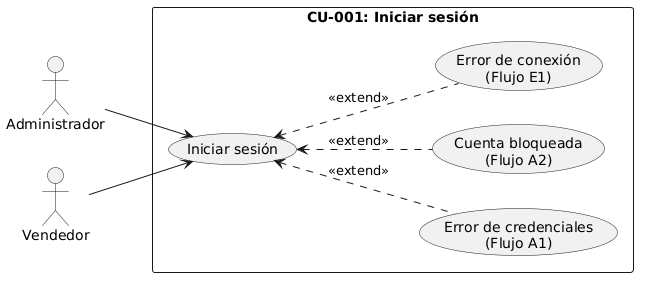
\includegraphics[width=0.9\textwidth]{doc/imagenes/Diagrama_de_Casos_de_Uso_CU001.png} 

\newpage
%==================== CU-002 ====================
\subsection{CU-002: Registrar producto}
\begin{center}
\begin{tabular}{
  |>{\centering\arraybackslash}m{4cm}|
   >{\centering\arraybackslash}m{5cm}|
   >{\centering\arraybackslash}m{4cm}|
   >{\centering\arraybackslash}m{3cm}|
}
\hline
\textbf{Código de caso de uso} & CU-002 & \textbf{Nombre del Caso de Uso} & Registrar producto \\
\hline
\textbf{Actor principal} & Administrador & & \\
\hline
\textbf{Actor Secundario} & Ninguno & & \\
\hline
\textbf{Descripción} & \multicolumn{3}{>{\centering\arraybackslash}m{12cm}|}{Permite al administrador registrar un nuevo producto con sus datos básicos y su stock inicial.} \\
\hline
\textbf{Precondiciones} & \multicolumn{3}{>{\centering\arraybackslash}m{12cm}|}{El usuario debe haber iniciado sesión con rol Administrador (CU-001). \newline Debe existir al menos una categoría registrada (CU-012).} \\
\hline
\textbf{Postcondiciones} & \multicolumn{3}{>{\centering\arraybackslash}m{12cm}|}{El producto queda registrado con su stock inicial. \newline El sistema registra un movimiento de entrada con motivo ``Stock inicial''. \newline El producto aparece en la lista de productos (CU-006).} \\
\hline
\multicolumn{4}{|>{\centering\arraybackslash}m{15.7cm}|}{\textbf{Flujo Principal}} \\
\hline
\multicolumn{2}{|C{8cm}|}{\textbf{Acción del actor}}
& \multicolumn{2}{C{8cm}|}{\textbf{Respuesta del Sistema}} \\
\hline
\multicolumn{2}{|C{8cm}|}{1. Selecciona la opción ``Registrar producto'' (POST \texttt{/api/inventario/productos/}).}
& \multicolumn{2}{C{8cm}|}{Muestra el formulario de registro.} \\
\hline
\multicolumn{2}{|C{8cm}|}{2. Ingresa nombre, categoría, precio unitario, cantidad inicial y stock mínimo.}
& \multicolumn{2}{C{8cm}|}{Valida los campos: precio $\geq$ 0.01, cantidad inicial $\geq$ 1, stock mínimo $\geq$ 1 y nombre único.} \\
\hline
\multicolumn{2}{|C{8cm}|}{3. Confirma el registro.}
& \multicolumn{2}{C{8cm}|}{Guarda el producto, crea el movimiento de stock inicial y muestra un mensaje de éxito.} \\
\hline
\multicolumn{4}{|C{15.7cm}|}{\textbf{Flujos Alternativos}} \\
\hline
\multicolumn{2}{|C{8cm}|}{A1}
& \multicolumn{2}{C{8cm}|}{El nombre del producto ya existe. Muestra un mensaje de error y solicita otro nombre.} \\
\hline
\multicolumn{2}{|C{8cm}|}{A2}
& \multicolumn{2}{C{8cm}|}{El precio o la cantidad inicial no son válidos. Muestra un error de validación y bloquea el registro.} \\
\hline
\multicolumn{4}{|C{15.7cm}|}{\textbf{Flujos de Excepciones}} \\
\hline
\multicolumn{2}{|C{8cm}|}{E1}
& \multicolumn{2}{C{8cm}|}{Error al guardar en la base de datos. Muestra el mensaje ``No se pudo registrar el producto''.} \\
\hline
\textbf{RF asociados} & RF-01, RF-04 & \textbf{RNF asociados} & RNF-01, RNF-04 \\
\hline
\end{tabular}
\end{center}

\newpage
\subsection*{Diagrama de caso de uso ``CU002''}
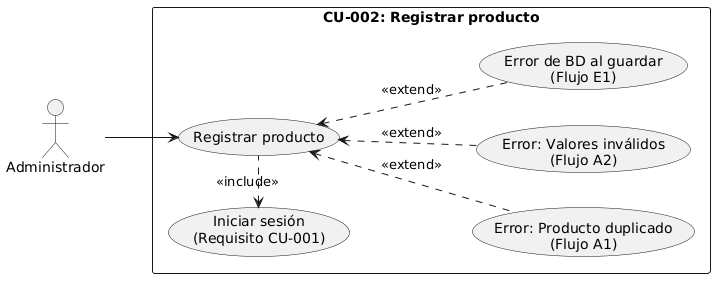
\includegraphics[width=0.9\textwidth]{doc/imagenes/Diagrama_de_Casos_de_Uso_CU002.png} 

\newpage
%==================== CU-003 ====================
\subsection{CU-003: Registrar entrada de stock}
\begin{center}
\begin{tabular}{
  |>{\centering\arraybackslash}m{4cm}|
   >{\centering\arraybackslash}m{5cm}|
   >{\centering\arraybackslash}m{4cm}|
   >{\centering\arraybackslash}m{3cm}|
}
\hline
\textbf{Código de caso de uso} & CU-003 & \textbf{Nombre del Caso de Uso} & Registrar entrada de stock \\
\hline
\textbf{Actor principal} & Administrador & & \\
\hline
\textbf{Actor Secundario} & Proveedor (externo) & & \\
\hline
\textbf{Descripción} & \multicolumn{3}{>{\centering\arraybackslash}m{12cm}|}{Permite registrar una compra a proveedor, incrementando el stock del producto seleccionado.} \\
\hline
\textbf{Precondiciones} & \multicolumn{3}{>{\centering\arraybackslash}m{12cm}|}{El usuario debe haber iniciado sesión con rol Administrador (CU-001). \newline El producto debe existir (CU-002) y el proveedor debe existir y estar activo.} \\
\hline
\textbf{Postcondiciones} & \multicolumn{3}{>{\centering\arraybackslash}m{12cm}|}{Se registra un movimiento de entrada con motivo ``Compra a proveedor'', fecha, hora, cantidad y proveedor. \newline Se recalcula el stock del producto.} \\
\hline
\multicolumn{4}{|>{\centering\arraybackslash}m{15.7cm}|}{\textbf{Flujo Principal}} \\
\hline
\multicolumn{2}{|C{8cm}|}{\textbf{Acción del actor}}
& \multicolumn{2}{C{8cm}|}{\textbf{Respuesta del Sistema}} \\
\hline
\multicolumn{2}{|C{8cm}|}{1. Selecciona ``Registrar entrada de stock'' (POST \texttt{/api/inventario/movimiento/entrada/}).}
& \multicolumn{2}{C{8cm}|}{Muestra el formulario de entrada.} \\
\hline
\multicolumn{2}{|C{8cm}|}{2. Selecciona el producto.}
& \multicolumn{2}{C{8cm}|}{Muestra el stock actual del producto.} \\
\hline
\multicolumn{2}{|C{8cm}|}{3. Ingresa la cantidad y selecciona el proveedor.}
& \multicolumn{2}{C{8cm}|}{Valida que la cantidad sea mayor a cero.} \\
\hline
\multicolumn{2}{|C{8cm}|}{4. Confirma la entrada.}
& \multicolumn{2}{C{8cm}|}{Registra el movimiento, recalcula el stock y muestra el nuevo stock.} \\
\hline
\multicolumn{4}{|C{15.7cm}|}{\textbf{Flujos Alternativos}} \\
\hline
\multicolumn{2}{|C{8cm}|}{A1}
& \multicolumn{2}{C{8cm}|}{La cantidad es cero o negativa. Muestra el mensaje ``La cantidad debe ser mayor a cero''.} \\
\hline
\multicolumn{2}{|C{8cm}|}{A2}
& \multicolumn{2}{C{8cm}|}{Producto o proveedor no encontrado. Muestra un mensaje de error y permite reintentar.} \\
\hline
\multicolumn{4}{|C{15.7cm}|}{\textbf{Flujos de Excepciones}} \\
\hline
\multicolumn{2}{|C{8cm}|}{E1}
& \multicolumn{2}{C{8cm}|}{Error al registrar el movimiento. La operación es atómica y no se aplica.} \\
\hline
\textbf{RF asociados} & RF-02, RF-04 & \textbf{RNF asociados} & RNF-03, RNF-04 \\
\hline
\end{tabular}
\end{center}

\newpage
\subsection*{Diagrama de caso de uso ``CU003''}
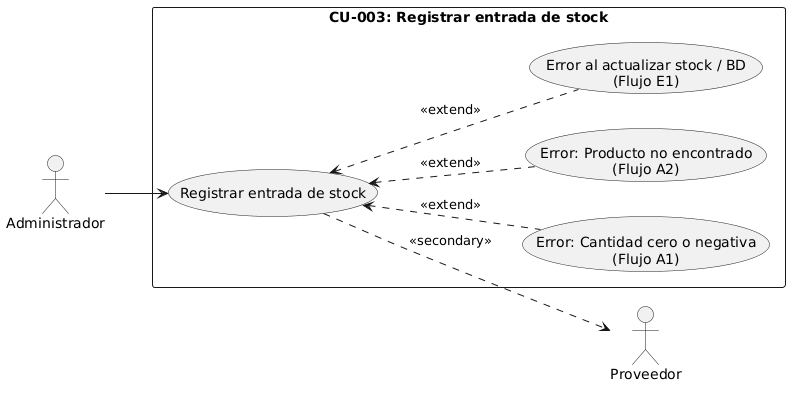
\includegraphics[width=0.9\textwidth]{doc/imagenes/Diagrama_de_Casos_de_Uso_CU003.png} 

\newpage
%==================== CU-005 ====================
\subsection{CU-005: Mostrar alerta de stock bajo}
\begin{center}
\begin{tabular}{
  |>{\centering\arraybackslash}m{4cm}|
   >{\centering\arraybackslash}m{5cm}|
   >{\centering\arraybackslash}m{4cm}|
   >{\centering\arraybackslash}m{3cm}|
}
\hline
\textbf{Código de caso de uso} & CU-005 & \textbf{Nombre del Caso de Uso} & Mostrar alerta de stock bajo \\
\hline
\textbf{Actor principal} & Sistema & & \\
\hline
\textbf{Actor Secundario} & Administrador, Vendedor & & \\
\hline
\textbf{Descripción} & \multicolumn{3}{>{\centering\arraybackslash}m{12cm}|}{El sistema muestra una alerta visual cuando el stock de un producto es igual o inferior al mínimo configurado.} \\
\hline
\textbf{Precondiciones} & \multicolumn{3}{>{\centering\arraybackslash}m{12cm}|}{El producto debe estar activo y tener configurado un stock mínimo.} \\
\hline
\textbf{Postcondiciones} & \multicolumn{3}{>{\centering\arraybackslash}m{12cm}|}{El producto aparece marcado visualmente en el panel principal mientras esté en alerta.} \\
\hline
\multicolumn{4}{|>{\centering\arraybackslash}m{15.7cm}|}{\textbf{Flujo Principal}} \\
\hline
\multicolumn{2}{|C{8cm}|}{\textbf{Acción del actor}}
& \multicolumn{2}{C{8cm}|}{\textbf{Respuesta del Sistema}} \\
\hline
\multicolumn{2}{|C{8cm}|}{1. El sistema consulta los productos en alerta (GET \texttt{/api/inventario/productos/alertas/}).}
& \multicolumn{2}{C{8cm}|}{Calcula el stock de cada producto a partir de sus movimientos.} \\
\hline
\multicolumn{2}{|C{8cm}|}{2. El sistema detecta stock menor o igual al mínimo.}
& \multicolumn{2}{C{8cm}|}{Devuelve y marca los productos en alerta en el panel principal.} \\
\hline
\multicolumn{4}{|C{15.7cm}|}{\textbf{Flujos Alternativos}} \\
\hline
\multicolumn{2}{|C{8cm}|}{A1}
& \multicolumn{2}{C{8cm}|}{El stock vuelve a estar por encima del mínimo. El producto deja de aparecer en la alerta.} \\
\hline
\multicolumn{4}{|C{15.7cm}|}{\textbf{Flujos de Excepciones}} \\
\hline
\multicolumn{2}{|C{8cm}|}{E1}
& \multicolumn{2}{C{8cm}|}{Error al calcular las alertas. Muestra el mensaje ``No se pudieron cargar las alertas''.} \\
\hline
\textbf{RF asociados} & RF-05 & \textbf{RNF asociados} & RNF-01, RNF-03 \\
\hline
\end{tabular}
\end{center}

\newpage
\subsection*{Diagrama de caso de uso ``CU005''}
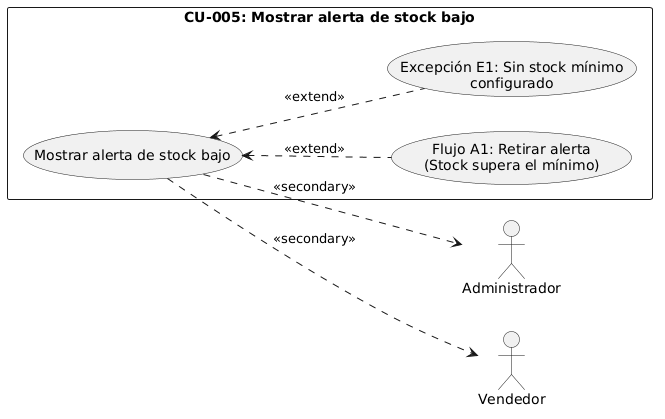
\includegraphics[width=0.9\textwidth]{doc/imagenes/Diagrama_de_Casos_de_Uso_CU005.png} 

\newpage
%==================== CU-006 ====================
\subsection{CU-006: Consultar lista de productos}
\begin{center}
\begin{tabular}{
  |>{\centering\arraybackslash}m{4cm}|
   >{\centering\arraybackslash}m{5cm}|
   >{\centering\arraybackslash}m{4cm}|
   >{\centering\arraybackslash}m{3cm}|
}
\hline
\textbf{Código de caso de uso} & CU-006 & \textbf{Nombre del Caso de Uso} & Consultar lista de productos \\
\hline
\textbf{Actor principal} & Administrador / Vendedor & & \\
\hline
\textbf{Actor Secundario} & Ninguno & & \\
\hline
\textbf{Descripción} & \multicolumn{3}{>{\centering\arraybackslash}m{12cm}|}{Permite consultar la lista de productos con su stock calculado.} \\
\hline
\textbf{Precondiciones} & \multicolumn{3}{>{\centering\arraybackslash}m{12cm}|}{El usuario debe haber iniciado sesión (CU-001).} \\
\hline
\textbf{Postcondiciones} & \multicolumn{3}{>{\centering\arraybackslash}m{12cm}|}{Se muestra la lista de productos con su stock actual. \newline No se modifica información del sistema.} \\
\hline
\multicolumn{4}{|>{\centering\arraybackslash}m{15.7cm}|}{\textbf{Flujo Principal}} \\
\hline
\multicolumn{2}{|C{8cm}|}{\textbf{Acción del actor}}
& \multicolumn{2}{C{8cm}|}{\textbf{Respuesta del Sistema}} \\
\hline
\multicolumn{2}{|C{8cm}|}{1. Selecciona ``Inventario'' (GET \texttt{/api/inventario/productos/select\_all/}).}
& \multicolumn{2}{C{8cm}|}{Recupera y muestra la lista de productos con su stock calculado.} \\
\hline
\multicolumn{2}{|C{8cm}|}{2. Recorre la lista.}
& \multicolumn{2}{C{8cm}|}{Muestra nombre, categoría, precio, stock y stock mínimo.} \\
\hline
\multicolumn{4}{|C{15.7cm}|}{\textbf{Flujos Alternativos}} \\
\hline
\multicolumn{2}{|C{8cm}|}{A1}
& \multicolumn{2}{C{8cm}|}{No hay productos registrados. Muestra el mensaje ``No hay productos registrados''.} \\
\hline
\multicolumn{4}{|C{15.7cm}|}{\textbf{Flujos de Excepciones}} \\
\hline
\multicolumn{2}{|C{8cm}|}{E1}
& \multicolumn{2}{C{8cm}|}{Error al recuperar los productos. Muestra el mensaje ``No se pudo cargar la lista''.} \\
\hline
\textbf{RF asociados} & RF-06 & \textbf{RNF asociados} & RNF-03 \\
\hline
\end{tabular}
\end{center}

\newpage
\subsection*{Diagrama de caso de uso ``CU006''}
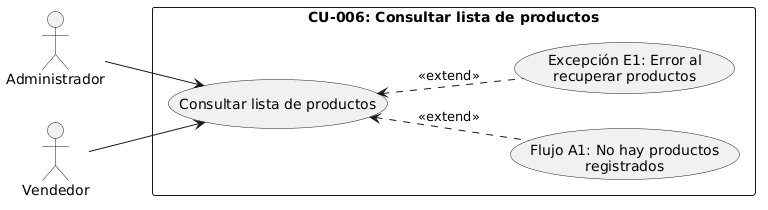
\includegraphics[width=0.9\textwidth]{doc/imagenes/Diagrama_de_Casos_de_Uso_CU006.png} 

\newpage
%==================== CU-007 ====================
\subsection{CU-007: Filtrar productos}
\begin{center}
\begin{tabular}{
  |>{\centering\arraybackslash}m{4cm}|
   >{\centering\arraybackslash}m{5cm}|
   >{\centering\arraybackslash}m{4cm}|
   >{\centering\arraybackslash}m{3cm}|
}
\hline
\textbf{Código de caso de uso} & CU-007 & \textbf{Nombre del Caso de Uso} & Filtrar productos \\
\hline
\textbf{Actor principal} & Administrador / Vendedor & & \\
\hline
\textbf{Actor Secundario} & Ninguno & & \\
\hline
\textbf{Descripción} & \multicolumn{3}{>{\centering\arraybackslash}m{12cm}|}{Permite filtrar los productos ya cargados por categoría, nombre y estado de stock (disponible, bajo, agotado).} \\
\hline
\textbf{Precondiciones} & \multicolumn{3}{>{\centering\arraybackslash}m{12cm}|}{El usuario debe haber iniciado sesión (CU-001). \newline Debe existir al menos un producto registrado.} \\
\hline
\textbf{Postcondiciones} & \multicolumn{3}{>{\centering\arraybackslash}m{12cm}|}{Se muestra la lista filtrada según los criterios seleccionados.} \\
\hline
\multicolumn{4}{|>{\centering\arraybackslash}m{15.7cm}|}{\textbf{Flujo Principal}} \\
\hline
\multicolumn{2}{|C{8cm}|}{\textbf{Acción del actor}}
& \multicolumn{2}{C{8cm}|}{\textbf{Respuesta del Sistema}} \\
\hline
\multicolumn{2}{|C{8cm}|}{1. Selecciona ``Filtrar productos''.}
& \multicolumn{2}{C{8cm}|}{Muestra las opciones de filtro.} \\
\hline
\multicolumn{2}{|C{8cm}|}{2. Ingresa categoría, nombre y/o estado.}
& \multicolumn{2}{C{8cm}|}{Aplica los filtros sobre la lista cargada y muestra los resultados.} \\
\hline
\multicolumn{4}{|C{15.7cm}|}{\textbf{Flujos Alternativos}} \\
\hline
\multicolumn{2}{|C{8cm}|}{A1}
& \multicolumn{2}{C{8cm}|}{Sin resultados. Muestra el mensaje ``No se encontraron productos con esos criterios''.} \\
\hline
\multicolumn{4}{|C{15.7cm}|}{\textbf{Flujos de Excepciones}} \\
\hline
\multicolumn{2}{|C{8cm}|}{E1}
& \multicolumn{2}{C{8cm}|}{Error al aplicar los filtros. Muestra el mensaje ``No se pudo aplicar el filtro''.} \\
\hline
\textbf{RF asociados} & RF-07 & \textbf{RNF asociados} & RNF-03 \\
\hline
\end{tabular}
\end{center}

\newpage
\subsection*{Diagrama de caso de uso ``CU007''}
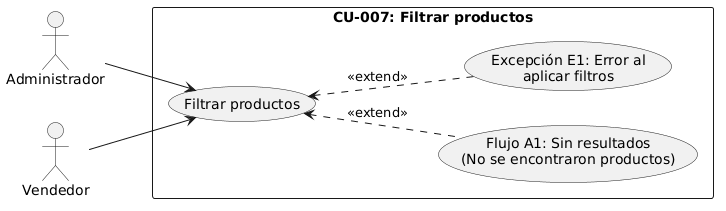
\includegraphics[width=0.9\textwidth]{doc/imagenes/Diagrama_de_Casos_de_Uso_CU007.png} 

\newpage
%==================== CU-008 ====================
\subsection{CU-008: Consultar historial de movimientos}
\begin{center}
\begin{tabular}{
  |>{\centering\arraybackslash}m{4cm}|
   >{\centering\arraybackslash}m{5cm}|
   >{\centering\arraybackslash}m{4cm}|
   >{\centering\arraybackslash}m{3cm}|
}
\hline
\textbf{Código de caso de uso} & CU-008 & \textbf{Nombre del Caso de Uso} & Consultar historial de movimientos \\
\hline
\textbf{Actor principal} & Administrador & & \\
\hline
\textbf{Actor Secundario} & Ninguno & & \\
\hline
\textbf{Descripción} & \multicolumn{3}{>{\centering\arraybackslash}m{12cm}|}{Permite consultar el historial de movimientos de stock (entradas y salidas), ordenado cronológicamente.} \\
\hline
\textbf{Precondiciones} & \multicolumn{3}{>{\centering\arraybackslash}m{12cm}|}{El usuario debe haber iniciado sesión (CU-001).} \\
\hline
\textbf{Postcondiciones} & \multicolumn{3}{>{\centering\arraybackslash}m{12cm}|}{Se muestra el historial de movimientos. No se modifica información del sistema.} \\
\hline
\multicolumn{4}{|>{\centering\arraybackslash}m{15.7cm}|}{\textbf{Flujo Principal}} \\
\hline
\multicolumn{2}{|C{8cm}|}{\textbf{Acción del actor}}
& \multicolumn{2}{C{8cm}|}{\textbf{Respuesta del Sistema}} \\
\hline
\multicolumn{2}{|C{8cm}|}{1. Selecciona ``Historial'' (GET \texttt{/api/inventario/history\_movimientos/}).}
& \multicolumn{2}{C{8cm}|}{Recupera los movimientos de stock.} \\
\hline
\multicolumn{2}{|C{8cm}|}{2. Revisa el listado.}
& \multicolumn{2}{C{8cm}|}{Muestra fecha, categoría/producto, cantidad y proveedor cuando corresponde.} \\
\hline
\multicolumn{4}{|C{15.7cm}|}{\textbf{Flujos Alternativos}} \\
\hline
\multicolumn{2}{|C{8cm}|}{A1}
& \multicolumn{2}{C{8cm}|}{No hay movimientos. Muestra el mensaje ``No hay movimientos registrados''.} \\
\hline
\multicolumn{4}{|C{15.7cm}|}{\textbf{Flujos de Excepciones}} \\
\hline
\multicolumn{2}{|C{8cm}|}{E1}
& \multicolumn{2}{C{8cm}|}{Error al recuperar el historial. Muestra el mensaje ``No se pudo cargar el historial''.} \\
\hline
\textbf{RF asociados} & RF-08 & \textbf{RNF asociados} & RNF-03 \\
\hline
\end{tabular}
\end{center}

\newpage
\subsection*{Diagrama de caso de uso ``CU008''}
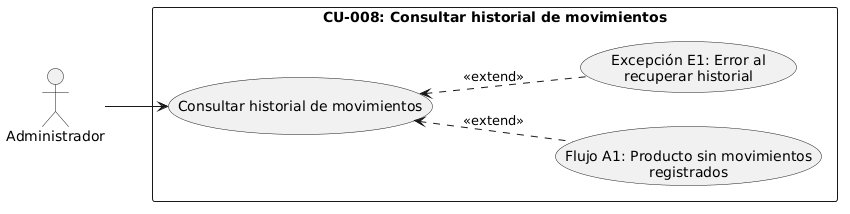
\includegraphics[width=0.9\textwidth]{doc/imagenes/Diagrama_de_Casos_de_Uso_CU008.png} 

\newpage
%==================== CU-011 ====================
\subsection{CU-011: Control de acceso según rol}
\begin{center}
\begin{tabular}{
  |>{\centering\arraybackslash}m{4cm}|
   >{\centering\arraybackslash}m{5cm}|
   >{\centering\arraybackslash}m{4cm}|
   >{\centering\arraybackslash}m{3cm}|
}
\hline
\textbf{Código de caso de uso} & CU-011 & \textbf{Nombre del Caso de Uso} & Control de acceso según rol \\
\hline
\textbf{Actor principal} & Sistema & & \\
\hline
\textbf{Actor Secundario} & Administrador, Vendedor & & \\
\hline
\textbf{Descripción} & \multicolumn{3}{>{\centering\arraybackslash}m{12cm}|}{El sistema dirige a cada usuario a un panel distinto según su rol y restringe las secciones de gestión al Administrador.} \\
\hline
\textbf{Precondiciones} & \multicolumn{3}{>{\centering\arraybackslash}m{12cm}|}{El usuario debe haber iniciado sesión (CU-001).} \\
\hline
\textbf{Postcondiciones} & \multicolumn{3}{>{\centering\arraybackslash}m{12cm}|}{El Administrador accede a todas las secciones; el Vendedor accede solo a Inicio e Inventario.} \\
\hline
\multicolumn{4}{|>{\centering\arraybackslash}m{15.7cm}|}{\textbf{Flujo Principal}} \\
\hline
\multicolumn{2}{|C{8cm}|}{\textbf{Acción del actor}}
& \multicolumn{2}{C{8cm}|}{\textbf{Respuesta del Sistema}} \\
\hline
\multicolumn{2}{|C{8cm}|}{1. El usuario inicia sesión.}
& \multicolumn{2}{C{8cm}|}{Lee el rol contenido en el token y determina el panel a mostrar.} \\
\hline
\multicolumn{2}{|C{8cm}|}{2. El sistema detecta el rol.}
& \multicolumn{2}{C{8cm}|}{Redirige al panel de Administrador o de Vendedor según corresponda.} \\
\hline
\multicolumn{4}{|C{15.7cm}|}{\textbf{Flujos Alternativos}} \\
\hline
\multicolumn{2}{|C{8cm}|}{A1}
& \multicolumn{2}{C{8cm}|}{Petición a la API sin token válido. El sistema responde con error de autenticación (401).} \\
\hline
\multicolumn{4}{|C{15.7cm}|}{\textbf{Flujos de Excepciones}} \\
\hline
\multicolumn{2}{|C{8cm}|}{E1}
& \multicolumn{2}{C{8cm}|}{El rol no es reconocido. El sistema rechaza el acceso al panel.} \\
\hline
\textbf{RF asociados} & RF-11 & \textbf{RNF asociados} & RNF-02 \\
\hline
\end{tabular}
\end{center}

\newpage
\subsection*{Diagrama de caso de uso ``CU011''}
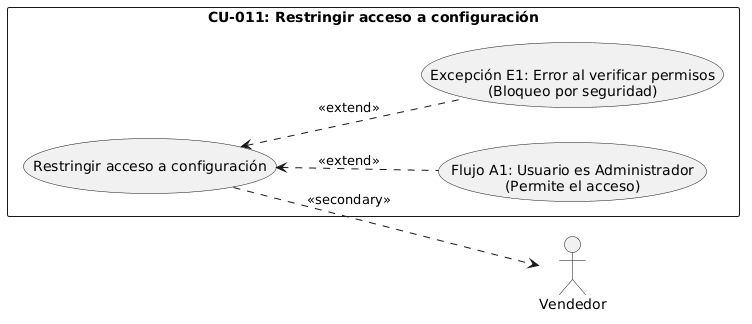
\includegraphics[width=0.9\textwidth]{doc/imagenes/Diagrama_de_Casos_de_Uso_CU011.png} 

\newpage
%==================== CU-012 ====================
\subsection{CU-012: Gestionar categorías de productos}
\begin{center}
\begin{tabular}{
  |>{\centering\arraybackslash}m{4cm}|
   >{\centering\arraybackslash}m{5cm}|
   >{\centering\arraybackslash}m{4cm}|
   >{\centering\arraybackslash}m{3cm}|
}
\hline
\textbf{Código de caso de uso} & CU-012 & \textbf{Nombre del Caso de Uso} & Gestionar categorías de productos \\
\hline
\textbf{Actor principal} & Administrador & & \\
\hline
\textbf{Actor Secundario} & Ninguno & & \\
\hline
\textbf{Descripción} & \multicolumn{3}{>{\centering\arraybackslash}m{12cm}|}{Permite al administrador registrar, listar, editar y eliminar categorías de productos.} \\
\hline
\textbf{Precondiciones} & \multicolumn{3}{>{\centering\arraybackslash}m{12cm}|}{El usuario debe haber iniciado sesión con rol Administrador (CU-001).} \\
\hline
\textbf{Postcondiciones} & \multicolumn{3}{>{\centering\arraybackslash}m{12cm}|}{La categoría queda registrada, actualizada o eliminada en el sistema.} \\
\hline
\multicolumn{4}{|>{\centering\arraybackslash}m{15.7cm}|}{\textbf{Flujo Principal}} \\
\hline
\multicolumn{2}{|C{8cm}|}{\textbf{Acción del actor}}
& \multicolumn{2}{C{8cm}|}{\textbf{Respuesta del Sistema}} \\
\hline
\multicolumn{2}{|C{8cm}|}{1. Selecciona ``Gestionar categorías'' (GET \texttt{/api/inventario/categorias/select/}).}
& \multicolumn{2}{C{8cm}|}{Muestra la lista de categorías.} \\
\hline
\multicolumn{2}{|C{8cm}|}{2. Selecciona ``Nueva categoría'' o edita una existente (POST \texttt{/api/inventario/add\_categoria/} o PUT \texttt{/api/inventario/categorias/\{pk\}/}).}
& \multicolumn{2}{C{8cm}|}{Muestra el formulario de categoría.} \\
\hline
\multicolumn{2}{|C{8cm}|}{3. Ingresa el nombre y confirma.}
& \multicolumn{2}{C{8cm}|}{Guarda la categoría y muestra un mensaje de éxito.} \\
\hline
\multicolumn{4}{|C{15.7cm}|}{\textbf{Flujos Alternativos}} \\
\hline
\multicolumn{2}{|C{8cm}|}{A1}
& \multicolumn{2}{C{8cm}|}{La categoría ya existe. Muestra el mensaje ``La categoría ya está registrada''.} \\
\hline
\multicolumn{2}{|C{8cm}|}{A2}
& \multicolumn{2}{|C{8cm}|}{Se intenta eliminar una categoría con productos asociados (DELETE \texttt{/api/inventario/categorias/\{pk\}/}). El sistema bloquea la eliminación.} \\
\hline
\multicolumn{4}{|C{15.7cm}|}{\textbf{Flujos de Excepciones}} \\
\hline
\multicolumn{2}{|C{8cm}|}{E1}
& \multicolumn{2}{C{8cm}|}{Error al guardar la categoría. Muestra el mensaje ``No se pudo guardar la categoría''.} \\
\hline
\textbf{RF asociados} & RF-12 & \textbf{RNF asociados} & RNF-04 \\
\hline
\end{tabular}
\end{center}

\newpage
\subsection*{Diagrama de caso de uso ``CU012''}
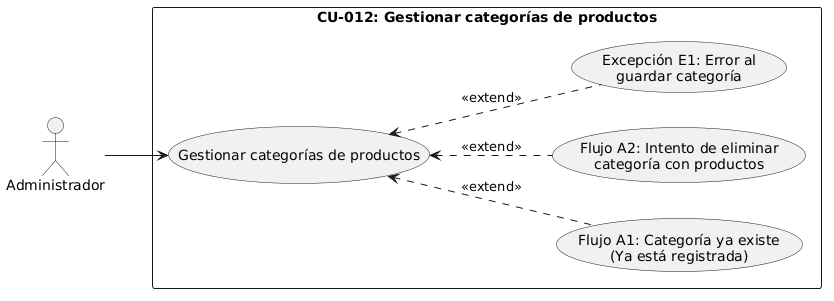
\includegraphics[width=0.9\textwidth]{doc/imagenes/Diagrama_de_Casos_de_Uso_CU012.png} 

\newpage
%==================== CU-013 ====================
\subsection{CU-013: Registrar usuario administrador}
\begin{center}
\begin{tabular}{
  |>{\centering\arraybackslash}m{4cm}|
   >{\centering\arraybackslash}m{5cm}|
   >{\centering\arraybackslash}m{4cm}|
   >{\centering\arraybackslash}m{3cm}|
}
\hline
\textbf{Código de caso de uso} & CU-013 & \textbf{Nombre del Caso de Uso} & Registrar usuario administrador \\
\hline
\textbf{Actor principal} & Usuario (registro público) & & \\
\hline
\textbf{Actor Secundario} & Ninguno & & \\
\hline
\textbf{Descripción} & \multicolumn{3}{>{\centering\arraybackslash}m{12cm}|}{Permite registrar un nuevo usuario con rol Administrador.} \\
\hline
\textbf{Precondiciones} & \multicolumn{3}{>{\centering\arraybackslash}m{12cm}|}{El correo no debe estar registrado.} \\
\hline
\textbf{Postcondiciones} & \multicolumn{3}{>{\centering\arraybackslash}m{12cm}|}{El usuario administrador queda registrado y habilitado para iniciar sesión (CU-001).} \\
\hline
\multicolumn{4}{|>{\centering\arraybackslash}m{15.7cm}|}{\textbf{Flujo Principal}} \\
\hline
\multicolumn{2}{|C{8cm}|}{\textbf{Acción del actor}}
& \multicolumn{2}{C{8cm}|}{\textbf{Respuesta del Sistema}} \\
\hline
\multicolumn{2}{|C{8cm}|}{1. Accede al registro de administrador (POST \texttt{/api/usuarios/registrar-admin/}).}
& \multicolumn{2}{C{8cm}|}{Muestra el formulario de registro.} \\
\hline
\multicolumn{2}{|C{8cm}|}{2. Ingresa nombre de usuario, correo y contraseña.}
& \multicolumn{2}{C{8cm}|}{Valida los campos obligatorios.} \\
\hline
\multicolumn{2}{|C{8cm}|}{3. Confirma el registro.}
& \multicolumn{2}{C{8cm}|}{Crea el usuario con rol Administrador y responde con su identificador.} \\
\hline
\multicolumn{4}{|C{15.7cm}|}{\textbf{Flujos Alternativos}} \\
\hline
\multicolumn{2}{|C{8cm}|}{A1}
& \multicolumn{2}{C{8cm}|}{El correo ya está registrado. Muestra un mensaje de error.} \\
\hline
\multicolumn{2}{|C{8cm}|}{A2}
& \multicolumn{2}{C{8cm}|}{Faltan campos obligatorios. El sistema indica los campos faltantes.} \\
\hline
\multicolumn{4}{|C{15.7cm}|}{\textbf{Flujos de Excepciones}} \\
\hline
\multicolumn{2}{|C{8cm}|}{E1}
& \multicolumn{2}{C{8cm}|}{Error al guardar el usuario. Muestra el mensaje ``No se pudo crear la cuenta''.} \\
\hline
\textbf{RF asociados} & RF-10 & \textbf{RNF asociados} & RNF-02 \\
\hline
\end{tabular}
\end{center}

\newpage
%==================== CU-014 ====================
\subsection{CU-014: Registrar usuario vendedor}
\begin{center}
\begin{tabular}{
  |>{\centering\arraybackslash}m{4cm}|
   >{\centering\arraybackslash}m{5cm}|
   >{\centering\arraybackslash}m{4cm}|
   >{\centering\arraybackslash}m{3cm}|
}
\hline
\textbf{Código de caso de uso} & CU-014 & \textbf{Nombre del Caso de Uso} & Registrar usuario vendedor \\
\hline
\textbf{Actor principal} & Administrador / Usuario (registro público) & & \\
\hline
\textbf{Actor Secundario} & Administrador existente & & \\
\hline
\textbf{Descripción} & \multicolumn{3}{>{\centering\arraybackslash}m{12cm}|}{Permite registrar un usuario con rol Vendedor, asociándolo a un Administrador existente.} \\
\hline
\textbf{Precondiciones} & \multicolumn{3}{>{\centering\arraybackslash}m{12cm}|}{El correo no debe estar registrado. \newline Debe existir un administrador con el nombre de usuario indicado.} \\
\hline
\textbf{Postcondiciones} & \multicolumn{3}{>{\centering\arraybackslash}m{12cm}|}{El vendedor queda registrado y asociado al Administrador, habilitado para iniciar sesión (CU-001).} \\
\hline
\multicolumn{4}{|>{\centering\arraybackslash}m{15.7cm}|}{\textbf{Flujo Principal}} \\
\hline
\multicolumn{2}{|C{8cm}|}{\textbf{Acción del actor}}
& \multicolumn{2}{C{8cm}|}{\textbf{Respuesta del Sistema}} \\
\hline
\multicolumn{2}{|C{8cm}|}{1. Accede al registro de vendedor (POST \texttt{/api/usuarios/registrar-vendedor/}).}
& \multicolumn{2}{C{8cm}|}{Muestra el formulario de registro.} \\
\hline
\multicolumn{2}{|C{8cm}|}{2. Ingresa nombre de usuario, correo, contraseña y el usuario del administrador.}
& \multicolumn{2}{C{8cm}|}{Valida que el administrador exista y sea Administrador.} \\
\hline
\multicolumn{2}{|C{8cm}|}{3. Confirma el registro.}
& \multicolumn{2}{C{8cm}|}{Crea el usuario con rol Vendedor asociado al Administrador.} \\
\hline
\multicolumn{4}{|C{15.7cm}|}{\textbf{Flujos Alternativos}} \\
\hline
\multicolumn{2}{|C{8cm}|}{A1}
& \multicolumn{2}{C{8cm}|}{El usuario administrador no existe. Muestra un mensaje de error.} \\
\hline
\multicolumn{2}{|C{8cm}|}{A2}
& \multicolumn{2}{C{8cm}|}{El correo ya está registrado. Muestra un mensaje de error.} \\
\hline
\multicolumn{4}{|C{15.7cm}|}{\textbf{Flujos de Excepciones}} \\
\hline
\multicolumn{2}{|C{8cm}|}{E1}
& \multicolumn{2}{C{8cm}|}{Error al guardar el usuario. Muestra un mensaje de error.} \\
\hline
\textbf{RF asociados} & RF-10 & \textbf{RNF asociados} & RNF-02 \\
\hline
\end{tabular}
\end{center}

\newpage
%==================== CU-015 ====================
\subsection{CU-015: Cerrar sesión}
\begin{center}
\begin{tabular}{
  |>{\centering\arraybackslash}m{4cm}|
   >{\centering\arraybackslash}m{5cm}|
   >{\centering\arraybackslash}m{4cm}|
   >{\centering\arraybackslash}m{3cm}|
}
\hline
\textbf{Código de caso de uso} & CU-015 & \textbf{Nombre del Caso de Uso} & Cerrar sesión \\
\hline
\textbf{Actor principal} & Administrador / Vendedor & & \\
\hline
\textbf{Actor Secundario} & Ninguno & & \\
\hline
\textbf{Descripción} & \multicolumn{3}{>{\centering\arraybackslash}m{12cm}|}{Permite finalizar la sesión eliminando los tokens almacenados en cookies.} \\
\hline
\textbf{Precondiciones} & \multicolumn{3}{>{\centering\arraybackslash}m{12cm}|}{El usuario debe haber iniciado sesión (CU-001).} \\
\hline
\textbf{Postcondiciones} & \multicolumn{3}{>{\centering\arraybackslash}m{12cm}|}{Las cookies de acceso y de refresco son eliminadas.} \\
\hline
\multicolumn{4}{|>{\centering\arraybackslash}m{15.7cm}|}{\textbf{Flujo Principal}} \\
\hline
\multicolumn{2}{|C{8cm}|}{\textbf{Acción del actor}}
& \multicolumn{2}{C{8cm}|}{\textbf{Respuesta del Sistema}} \\
\hline
\multicolumn{2}{|C{8cm}|}{1. Selecciona ``Cerrar sesión'' (POST \texttt{/api/usuarios/auth/logout/}).}
& \multicolumn{2}{C{8cm}|}{Elimina las cookies \texttt{access\_token} y \texttt{refresh\_token} y responde con éxito.} \\
\hline
\multicolumn{4}{|C{15.7cm}|}{\textbf{Flujos de Excepciones}} \\
\hline
\multicolumn{2}{|C{8cm}|}{E1}
& \multicolumn{2}{C{8cm}|}{Error al procesar la solicitud. Muestra un mensaje de error.} \\
\hline
\textbf{RF asociados} & RF-13 & \textbf{RNF asociados} & RNF-02 \\
\hline
\end{tabular}
\end{center}

\newpage
%==================== CU-016 ====================
\subsection{CU-016: Actualizar producto}
\begin{center}
\begin{tabular}{
  |>{\centering\arraybackslash}m{4cm}|
   >{\centering\arraybackslash}m{5cm}|
   >{\centering\arraybackslash}m{4cm}|
   >{\centering\arraybackslash}m{3cm}|
}
\hline
\textbf{Código de caso de uso} & CU-016 & \textbf{Nombre del Caso de Uso} & Actualizar producto \\
\hline
\textbf{Actor principal} & Administrador & & \\
\hline
\textbf{Actor Secundario} & Ninguno & & \\
\hline
\textbf{Descripción} & \multicolumn{3}{>{\centering\arraybackslash}m{12cm}|}{Permite modificar los datos de un producto existente (nombre, categoría, precio unitario y stock mínimo).} \\
\hline
\textbf{Precondiciones} & \multicolumn{3}{>{\centering\arraybackslash}m{12cm}|}{El usuario debe haber iniciado sesión con rol Administrador (CU-001). \newline El producto debe existir.} \\
\hline
\textbf{Postcondiciones} & \multicolumn{3}{>{\centering\arraybackslash}m{12cm}|}{Los datos del producto quedan actualizados y se reflejan en la lista (CU-006).} \\
\hline
\multicolumn{4}{|>{\centering\arraybackslash}m{15.7cm}|}{\textbf{Flujo Principal}} \\
\hline
\multicolumn{2}{|C{8cm}|}{\textbf{Acción del actor}}
& \multicolumn{2}{C{8cm}|}{\textbf{Respuesta del Sistema}} \\
\hline
\multicolumn{2}{|C{8cm}|}{1. Selecciona un producto y la opción ``Editar''.}
& \multicolumn{2}{C{8cm}|}{Carga los datos del producto en el formulario.} \\
\hline
\multicolumn{2}{|C{8cm}|}{2. Modifica los datos y confirma (PUT \texttt{/api/inventario/productos/\{pk\}/}).}
& \multicolumn{2}{C{8cm}|}{Valida y guarda los cambios, y muestra un mensaje de éxito.} \\
\hline
\multicolumn{4}{|C{15.7cm}|}{\textbf{Flujos Alternativos}} \\
\hline
\multicolumn{2}{|C{8cm}|}{A1}
& \multicolumn{2}{C{8cm}|}{El producto no existe. El sistema responde con error 404.} \\
\hline
\multicolumn{2}{|C{8cm}|}{A2}
& \multicolumn{2}{C{8cm}|}{Datos inválidos. Muestra un error de validación.} \\
\hline
\multicolumn{4}{|C{15.7cm}|}{\textbf{Flujos de Excepciones}} \\
\hline
\multicolumn{2}{|C{8cm}|}{E1}
& \multicolumn{2}{C{8cm}|}{Error al guardar los cambios. Muestra un mensaje de error.} \\
\hline
\textbf{RF asociados} & RF-03 & \textbf{RNF asociados} & RNF-04 \\
\hline
\end{tabular}
\end{center}

\newpage
%==================== CU-017 ====================
\subsection{CU-017: Consultar resumen del día}
\begin{center}
\begin{tabular}{
  |>{\centering\arraybackslash}m{4cm}|
   >{\centering\arraybackslash}m{5cm}|
   >{\centering\arraybackslash}m{4cm}|
   >{\centering\arraybackslash}m{3cm}|
}
\hline
\textbf{Código de caso de uso} & CU-017 & \textbf{Nombre del Caso de Uso} & Consultar resumen del día \\
\hline
\textbf{Actor principal} & Administrador / Vendedor & & \\
\hline
\textbf{Actor Secundario} & Ninguno & & \\
\hline
\textbf{Descripción} & \multicolumn{3}{>{\centering\arraybackslash}m{12cm}|}{Permite consultar los totales de entradas y salidas de stock del día actual.} \\
\hline
\textbf{Precondiciones} & \multicolumn{3}{>{\centering\arraybackslash}m{12cm}|}{El usuario debe haber iniciado sesión (CU-001).} \\
\hline
\textbf{Postcondiciones} & \multicolumn{3}{>{\centering\arraybackslash}m{12cm}|}{Se muestran los totales del día. No se modifica información del sistema.} \\
\hline
\multicolumn{4}{|>{\centering\arraybackslash}m{15.7cm}|}{\textbf{Flujo Principal}} \\
\hline
\multicolumn{2}{|C{8cm}|}{\textbf{Acción del actor}}
& \multicolumn{2}{C{8cm}|}{\textbf{Respuesta del Sistema}} \\
\hline
\multicolumn{2}{|C{8cm}|}{1. Ingresa al panel principal (GET \texttt{/api/inventario/resumen/hoy/}).}
& \multicolumn{2}{C{8cm}|}{Calcula el total de entradas y de salidas del día.} \\
\hline
\multicolumn{2}{|C{8cm}|}{2. Observa el resumen del día.}
& \multicolumn{2}{C{8cm}|}{Muestra la cantidad total de entradas y de salidas.} \\
\hline
\multicolumn{4}{|C{15.7cm}|}{\textbf{Flujos Alternativos}} \\
\hline
\multicolumn{2}{|C{8cm}|}{A1}
& \multicolumn{2}{C{8cm}|}{No hay movimientos en el día. Muestra 0 en ambos totales.} \\
\hline
\multicolumn{4}{|C{15.7cm}|}{\textbf{Flujos de Excepciones}} \\
\hline
\multicolumn{2}{|C{8cm}|}{E1}
& \multicolumn{2}{C{8cm}|}{Error al calcular el resumen. Muestra un mensaje de error.} \\
\hline
\textbf{RF asociados} & RF-09 & \textbf{RNF asociados} & RNF-03 \\
\hline
\end{tabular}
\end{center}

\newpage

% ================================ DIAGRAMA DE CLASES
\section{Diagrama de clases}
\subsection{El diagrama de clases de todo el programa}
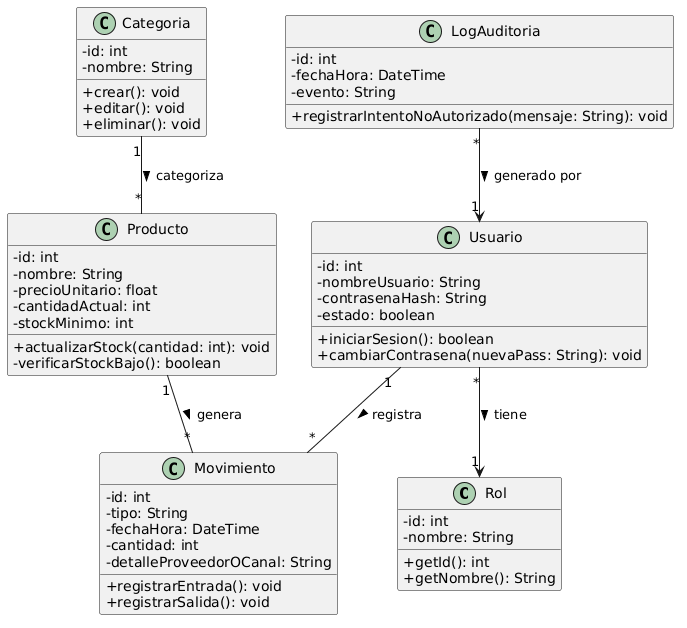
\includegraphics[width=0.9\textwidth]{doc/imagenes/Diagrama_de_Clases.png}
\newpage

% ================================ DIAGRAMA DE SECUENCIAS
\section{Diagrama de secuencias}

\needspace{30\baselineskip}
\subsection{CU-001: Iniciar sesión}
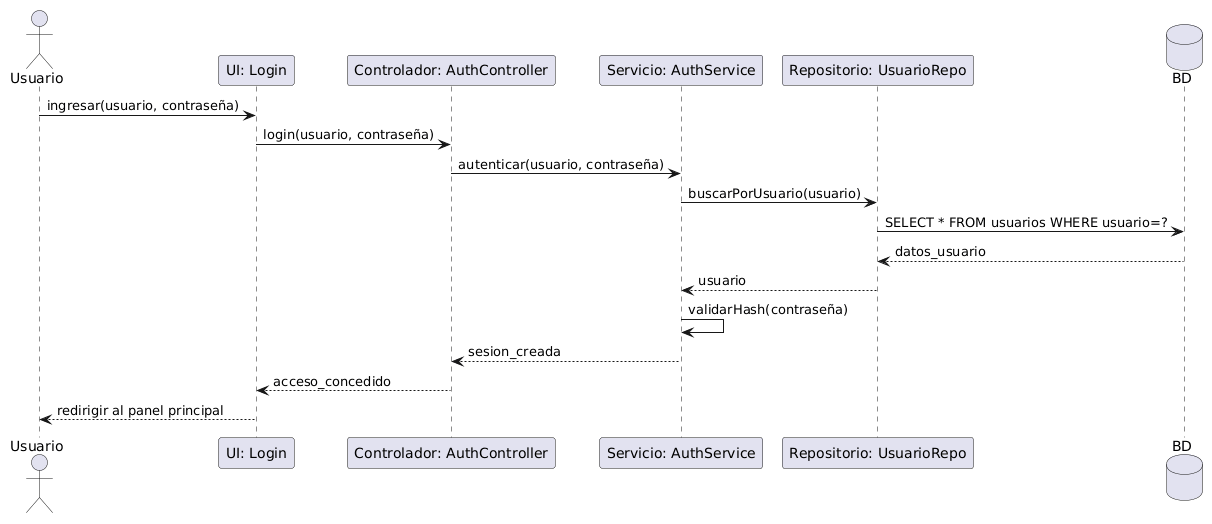
\includegraphics[width=0.9\textwidth]{doc/imagenes/Diagrama_de_Secuencias_CU001.png}

\needspace{30\baselineskip}
\subsection{CU-002: Registrar producto}
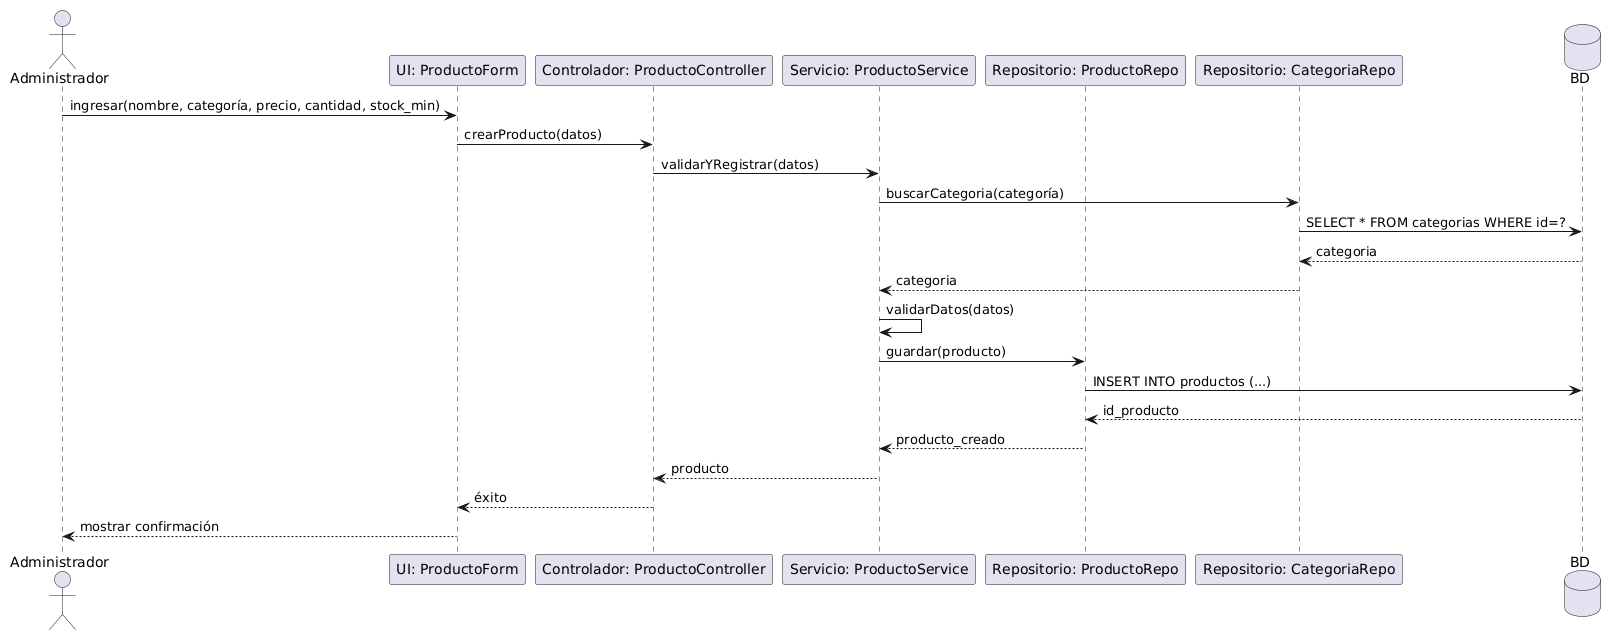
\includegraphics[width=0.9\textwidth]{doc/imagenes/Diagrama_de_Secuencias_CU002.png}

\needspace{30\baselineskip}
\subsection{CU-003: Registrar entrada de stock}
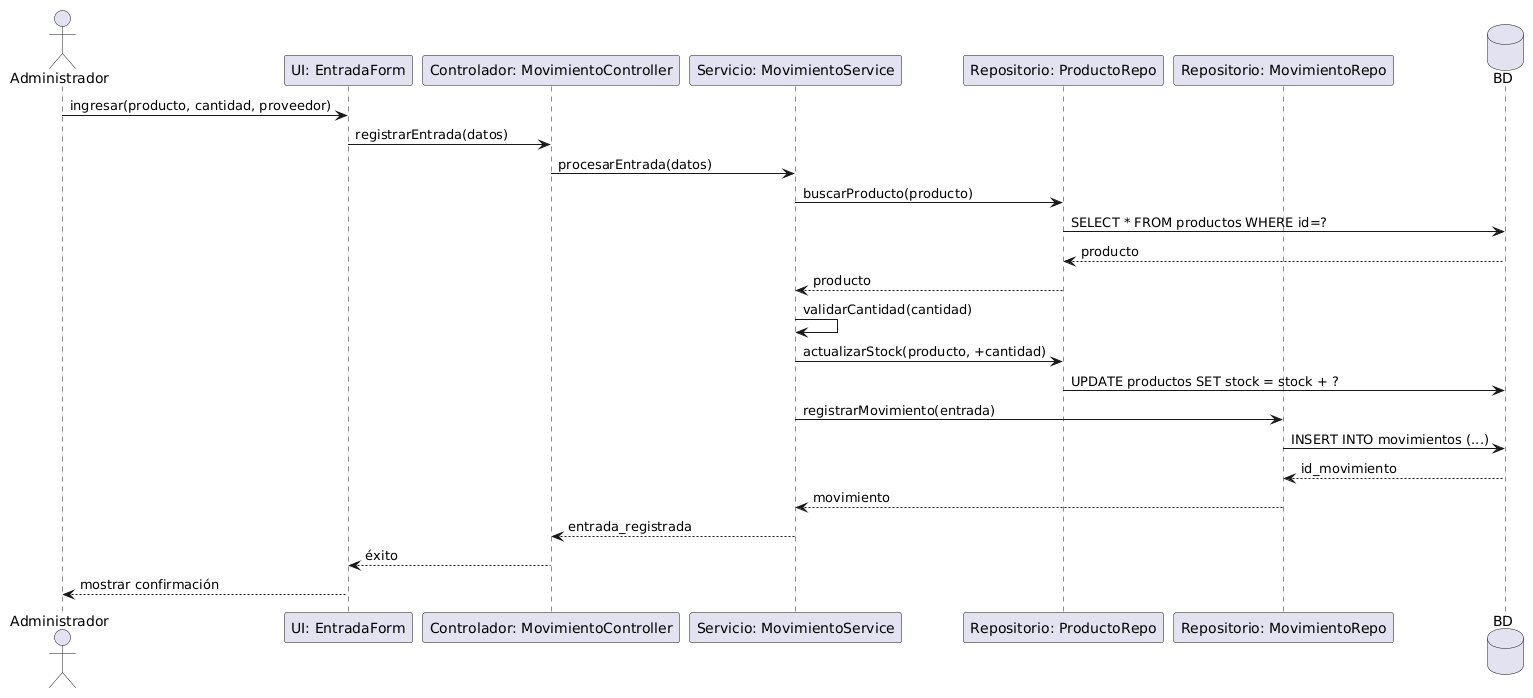
\includegraphics[width=0.9\textwidth]{doc/imagenes/Diagrama_de_Secuencias_CU003.png}

\needspace{30\baselineskip}
\subsection{CU-005: Mostrar alerta de stock bajo}
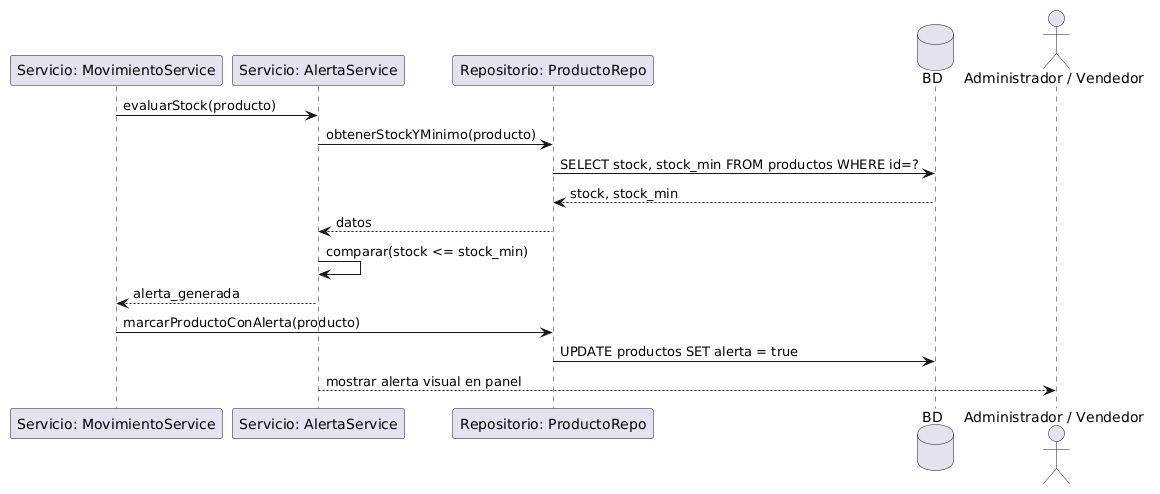
\includegraphics[width=0.9\textwidth]{doc/imagenes/Diagrama_de_Secuencias_CU005.png}

\needspace{30\baselineskip}
\subsection{CU-006: Consultar lista de productos}
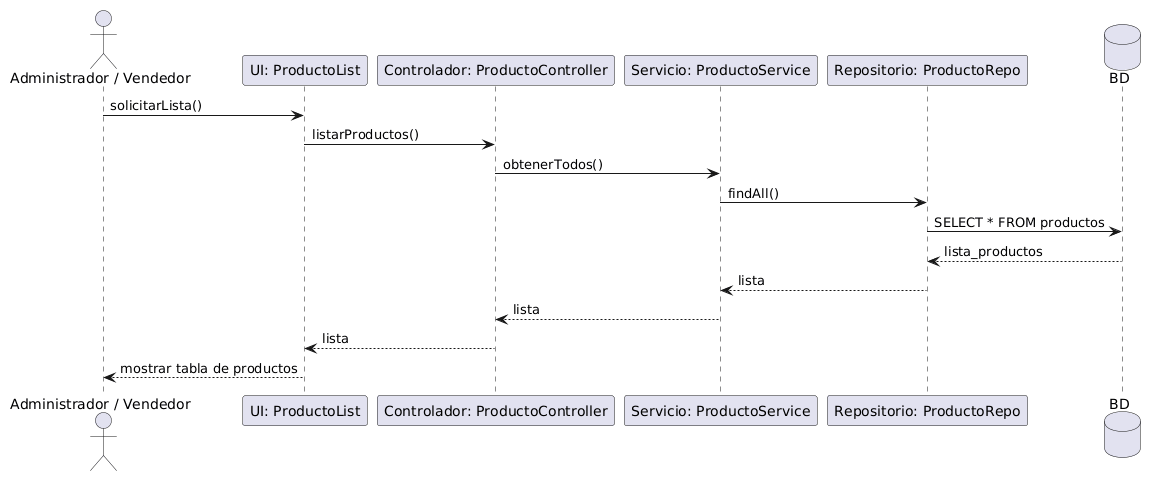
\includegraphics[width=0.9\textwidth]{doc/imagenes/Diagrama_de_Secuencias_CU006.png}

\needspace{30\baselineskip}
\subsection{CU-007: Filtrar productos}
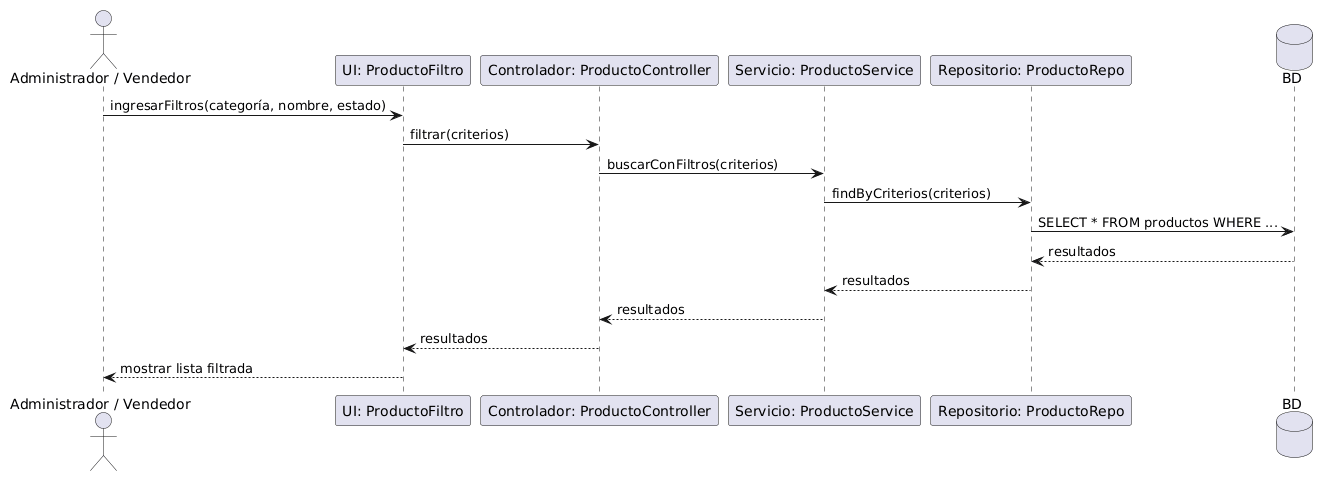
\includegraphics[width=0.9\textwidth]{doc/imagenes/Diagrama_de_Secuencias_CU007.png}

\needspace{30\baselineskip}
\subsection{CU-008: Consultar historial de movimientos}
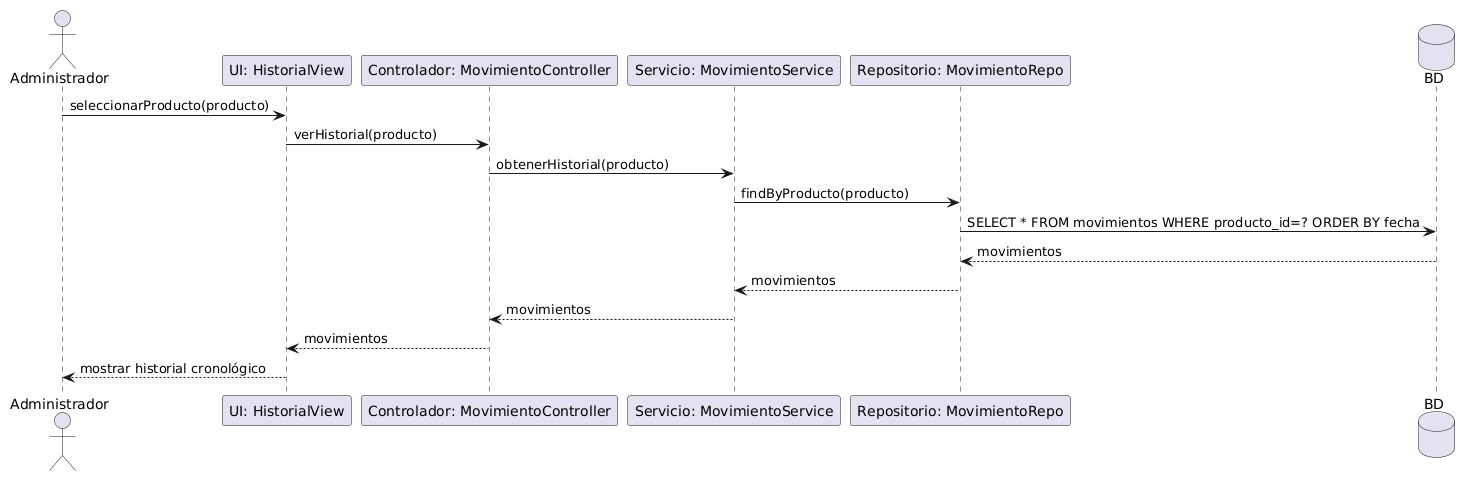
\includegraphics[width=0.9\textwidth]{doc/imagenes/Diagrama_de_Secuencias_CU008.png}

\needspace{30\baselineskip}
\subsection{CU-011: Control de acceso según rol}
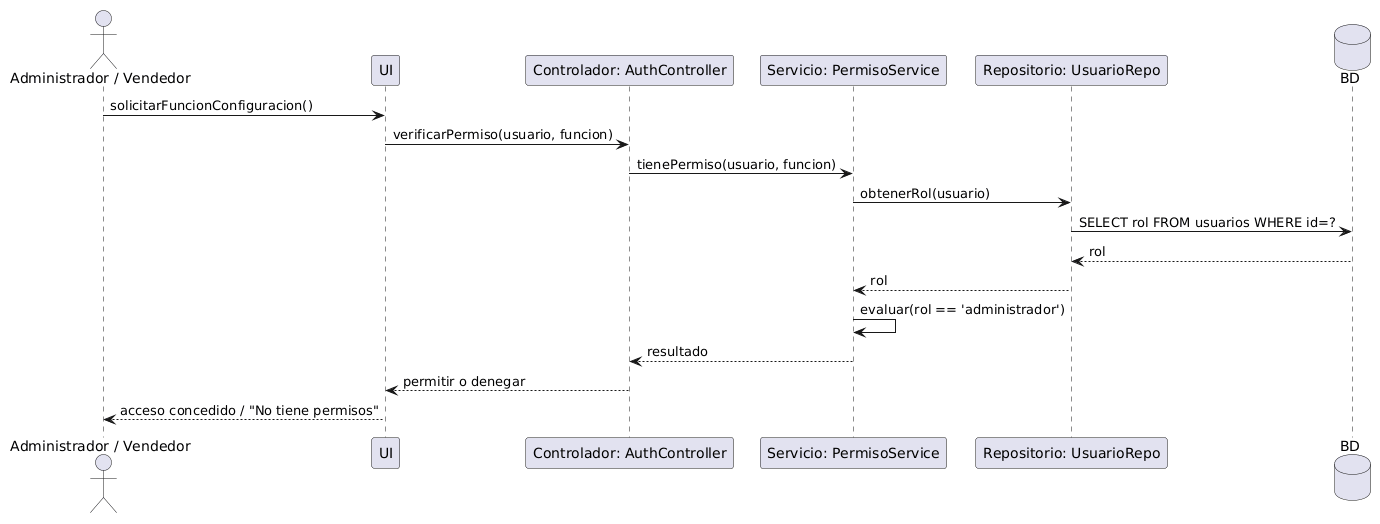
\includegraphics[width=0.9\textwidth]{doc/imagenes/Diagrama_de_Secuencias_CU011.png}

\needspace{30\baselineskip}
\subsection{CU-012: Gestionar categorías de productos}
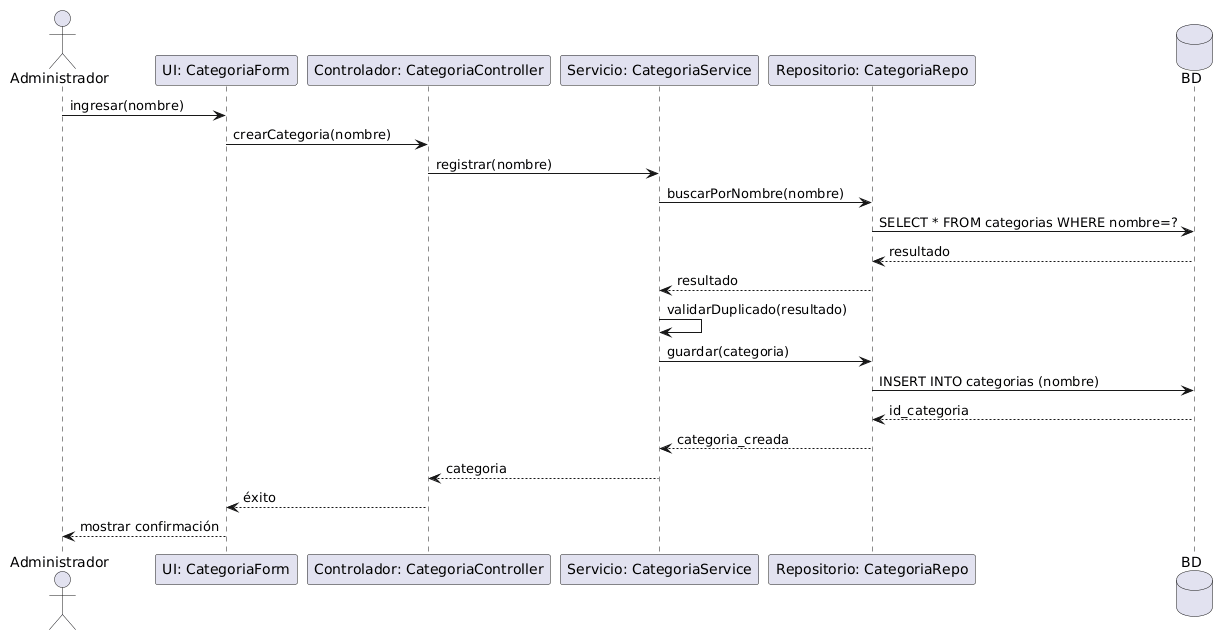
\includegraphics[width=0.9\textwidth]{doc/imagenes/Diagrama_de_Secuencias_CU012.png}

\newpage

% ================================ BACKLOG
\section{Backlog / Fuera del alcance del MVP}
Las siguientes funcionalidades no forman parte de la versión 1.0 y se priorizan con MoSCoW para
futuras iteraciones:

\begin{center}
\renewcommand{\arraystretch}{1.4}
\begin{tabular}{|L{5.5cm}|L{2.5cm}|L{8cm}|}
\hline
\textbf{Funcionalidad} & \textbf{Prioridad} & \textbf{Descripción} \\
\hline
Registrar salida / venta & Could & Registrar salidas de stock indicando el canal de venta (WhatsApp, redes, presencial, etc.). Existe el caso de uso en el dominio, pero no está expuesto por la API. \\
\hline
Canal de venta & Could & Campo de canal de venta por movimiento de salida (no está en el modelo de datos actual). \\
\hline
Estadísticas por período & Could & Productos más vendidos y resumen de movimientos por rango de fechas. \\
\hline
Gestión avanzada de usuarios & Could & Editar, activar/desactivar y cambiar el rol de los usuarios desde la interfaz. \\
\hline
CRUD de proveedores & Could & Crear, editar y eliminar proveedores por interfaz (hoy solo se listan los activos). \\
\hline
Configuración del sistema & Could & Parámetros del negocio (nombre, moneda u otros). \\
\hline
Notificaciones por correo o mensajería & Won't & Envío de alertas de stock por correo o mensajería. \\
\hline
Bloqueo por intentos fallidos y recuperación de contraseña & Won't & Bloqueo de cuenta tras varios intentos y restablecimiento de contraseña. \\
\hline
\end{tabular}
\end{center}

\end{document}
